\chapter{Plataforma OpenROV}
\label{cap:plataformaOpenROV}

\section{Robot Submarino OpenROV}
\label{cap:Robot Submarino OpenROV}
La robótica submarina lleva desarrollándose desde mediados de los años sesenta, aunque fuera una realidad desconocida para el gran público. Los robots submarinos costaban millones y tenían el tamaño de un todoterreno. Un robot con una cámara que se retransmite en directo a una página web. Su principal virtud es que OpenROV\footnote{https://www.openrov.com/} funciona con código abierto.

En general, sus características entran dentro de los parámetros presentados a continuación:

  \begin{itemize}
  \item \textbf{Cámara web de alta definición para video en vivo HD} Se transmite vídeo de alta definición a un portátil a través de un cable trenzado de dos hilos.
  \item \textbf{Tres servomotores} Se utilizan para la movilidad del dispositivo. Son de muy bajo mantenimiento y puedan estar en contacto directamente con el agua.
  \item \textbf{Flotabilidad neutra y altamente maniobrable} El diseño compacto y ligero permite una alta maniobrabilidad utilizando un diseño de tres actuadores. Se puede sumergir a una profundidad de 100 metros.
  \item \textbf{Interfaz web fácil de usar} En ella se puede manipular la cámara, los láser, focos y motores. No necesita conexión a Internet, ni hay necesidad de instalar un software.
  \item \textbf{Soporte de la comunidad de OpenROV} Se tiene soporte de la amplia comunidad que da soporte al proyecto OpenROV.
  \end{itemize}

\begin{figure}[hbtp]
  \begin{center}
    \subfigure[OpenROV parte frontal]{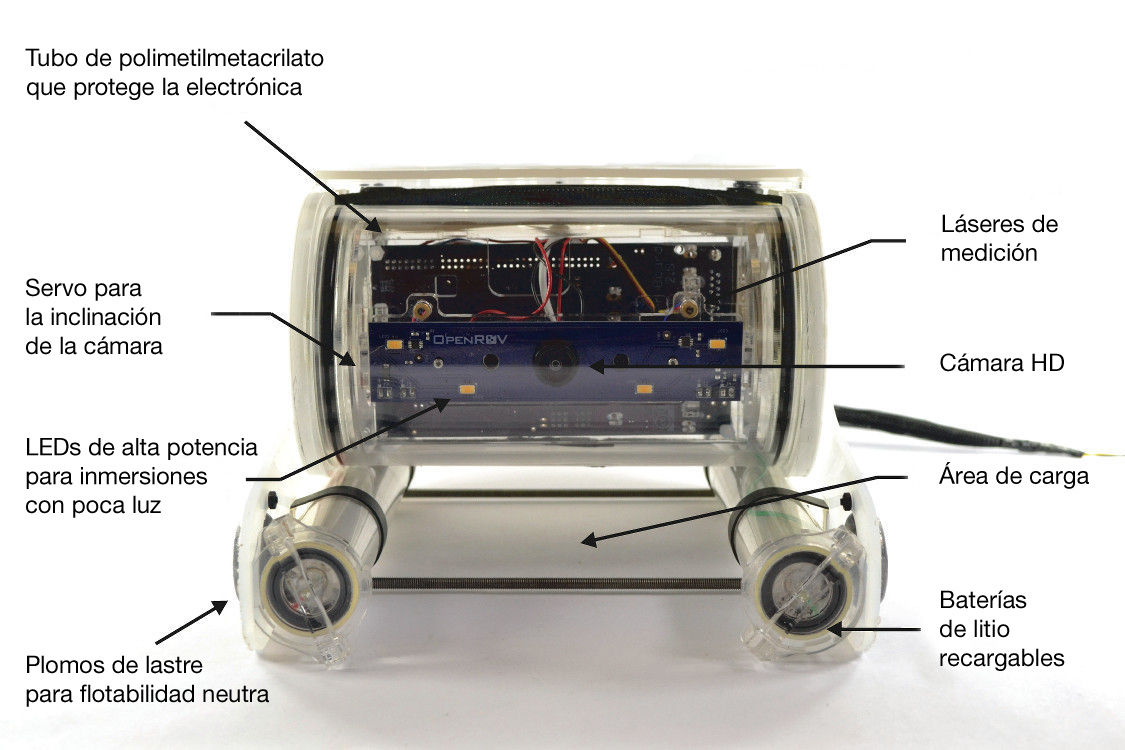
\includegraphics[width=6cm,height=5cm]{img/cap3/ROV_frontal}}
    \subfigure[OpenROV parte trasera]{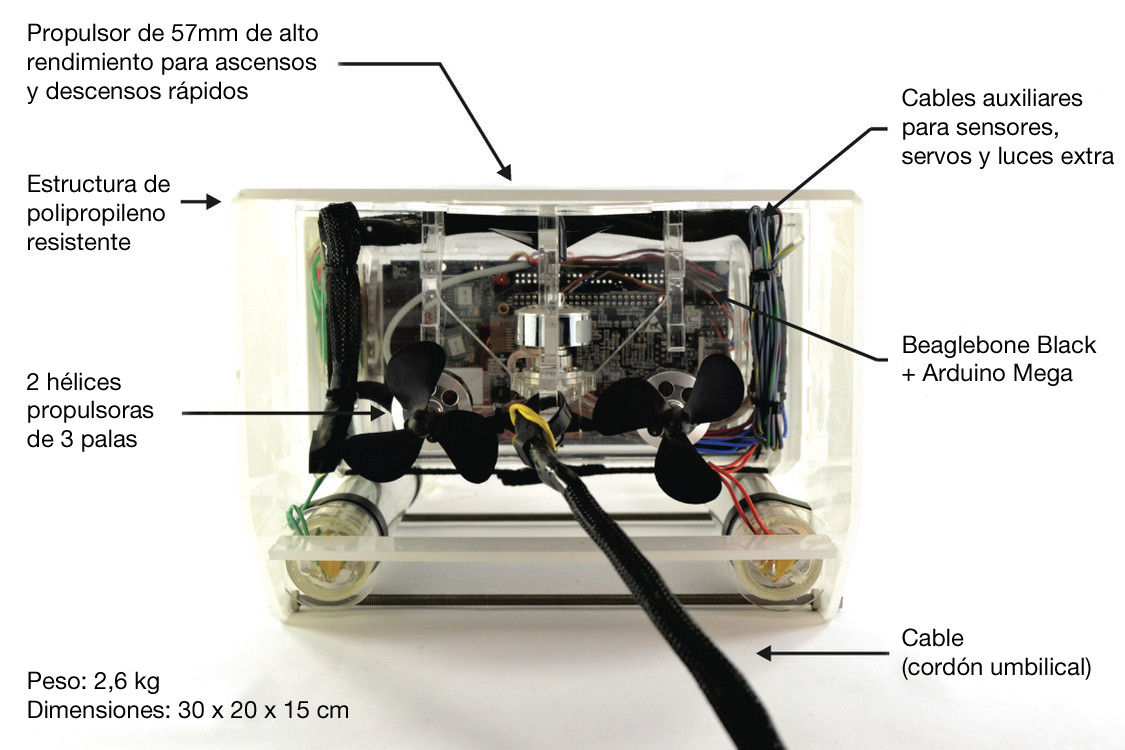
\includegraphics[width=6cm,height=5cm]{img/cap3/ROV_trasera}}
  \end{center}
  \caption{OpenROV}
  \label{fig:ROV-ej}
\end{figure}

\section{Estado del Arte}
\label{cap:Estado del Arte}
El mundo de los robots submarinos ROV (\textit{Remote Operated Vehicle} o vehículo de operación  remota) sigue creciendo año tras año y no debe sorprender. El 70\% por ciento de la superficie de la Tierra está cubierta de océanos. El 95\% del fondo de los océanos sigue sin mapear. De hecho, se conoce más sobre la superficie de la Luna que de las profundidades oceánicas. Tanto es así, que doce hombres han puesto pie en la Luna, pero sólo dos lo hicieron en la Fosa de las Marianas, la parte más profunda de nuestros mares, con aproximadamente 11 kilómetros de profundidad.

La inherente necesidad del ser humano de ir hacia lo desconocido para expandir nuestras fronteras no tiene límite. Esto se ve reflejado en el aumento de proyectos que buscan expandir estas fronteras submarinas.

En base al estudio del estado del arte, se establecieron las variables físicas necesarias para poder manipular el robot en cuestión, estas variables son las siguientes:
  \begin{itemize}
  \item \textbf{Aceleraciones en X, Y, Z} Permite obtener el ángulo con respecto al plano. Por odometría se puede obtener velocidad y posición estimadas.
  \item \textbf{Velocidad angular en p, q y r (roll, pitch y yaw)} Por medio de odometría, permite estimar perturbaciones en la rotación del robot.
  \item \textbf{Temperatura Externa} Puede utilizarse para hacer un registro de datos que permita caracterizar unmedio marino.
  \item \textbf{Temperatura Interna} Puede proveer de alerta de sobrecalentamiento de los sistemas a bordo.
  \item \textbf{Velocidades Lineales} En conjunto con la estimación de velocidad por odometría, puede utilizarse para compensar errores acumulativos.
  \item \textbf{Orientación con respecto al norte magnético} Permite obtener una referencia para mantener una referencia con respecto a la tierra.
  \item \textbf{Presión Relativa} De manera indirecta, permite conocer la profundidad.
  \item \textbf{Carga de Baterías} Permite conocer el estado de carga de las baterías. En caso de estar en un nivel crítico, se pueden ejecutar modos de bajo consumo o de recuperación de la plataforma.
  \end{itemize}

\section{Estructura y Montaje}
\label{cap:montaje}

\subsection{Estructura de OpenROV}
\label{subsec:EstructuraOpenROV}

Antes de comenzar con el montaje de la estructura, la cámara y el chasis del ROV, se necesitarán ciertas herramientas para el correcto ensamblaje.

Las herramientas necesarias son: guantes, gafas, cúter, cemento acrílico y pegamento. Una vez hayamos obtenido todos los materiales empezaremos con el montaje.

\begin{figure} [hbtp]
  \begin{center}
    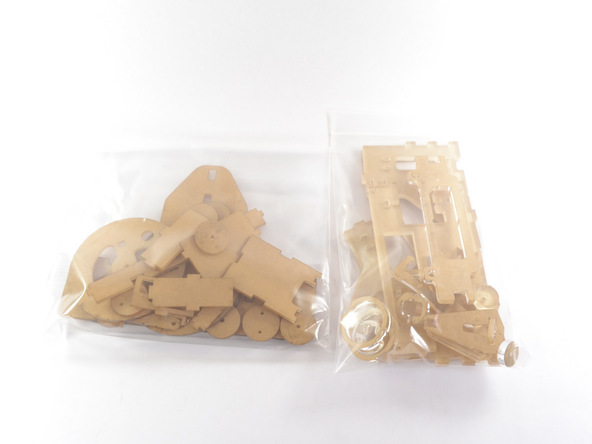
\includegraphics[width=8cm]{img/cap3/3_3/piezas}
  \end{center}
  \caption{Piezas de los chásis.}
  \label{fig:piezas}
\end{figure}

Se separan las piezas para realizar su correcto montaje. Una vez localizadas las piezas para la estructura, se le quitará el papel protector a la pieza, lo cual la dejará de un color trasparente. 
Iremos pegando y dejando secar para que la composición sea la correcta. 
Al final, quedará una estructura como la de la imagen.

\begin{figure} [hbtp]
  \begin{center}
    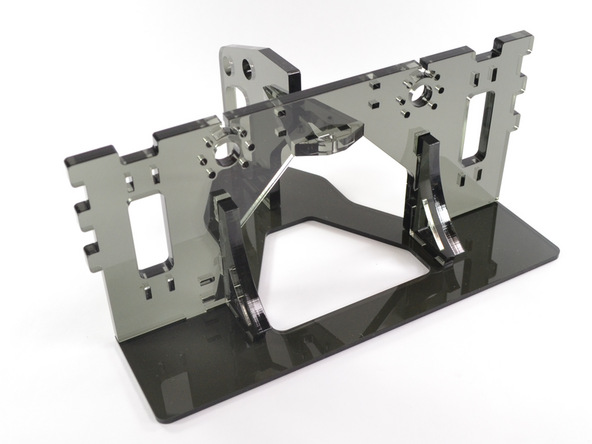
\includegraphics[width=8cm]{img/cap3/3_3/chasis_ppal}
  \end{center}
  \caption{Chasis principal.}
  \label{fig:chasis_ppal}
\end{figure}

Para el montaje de la estructura del soporte de la cámara y el chasis de la electrónica se realizará el mismo procedimiento que en el caso anterior, con un resultado como el de las siguientes fotos:

\begin{figure}[hbtp]
  \begin{center}
    \subfigure[Soporte de la cámara]{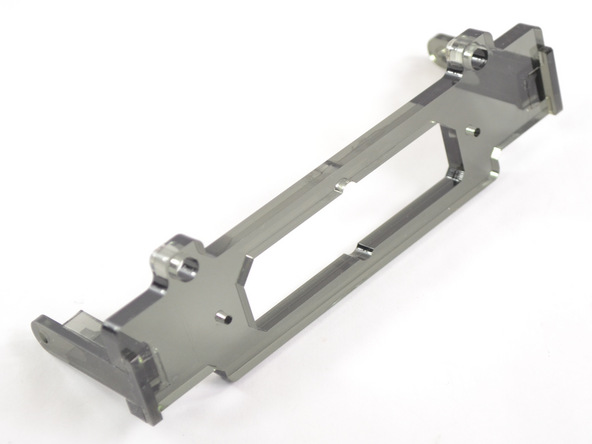
\includegraphics[width=6cm,height=5cm]{img/cap3/3_3/chasis_camara}}
    \subfigure[Chasis de la electrónica]{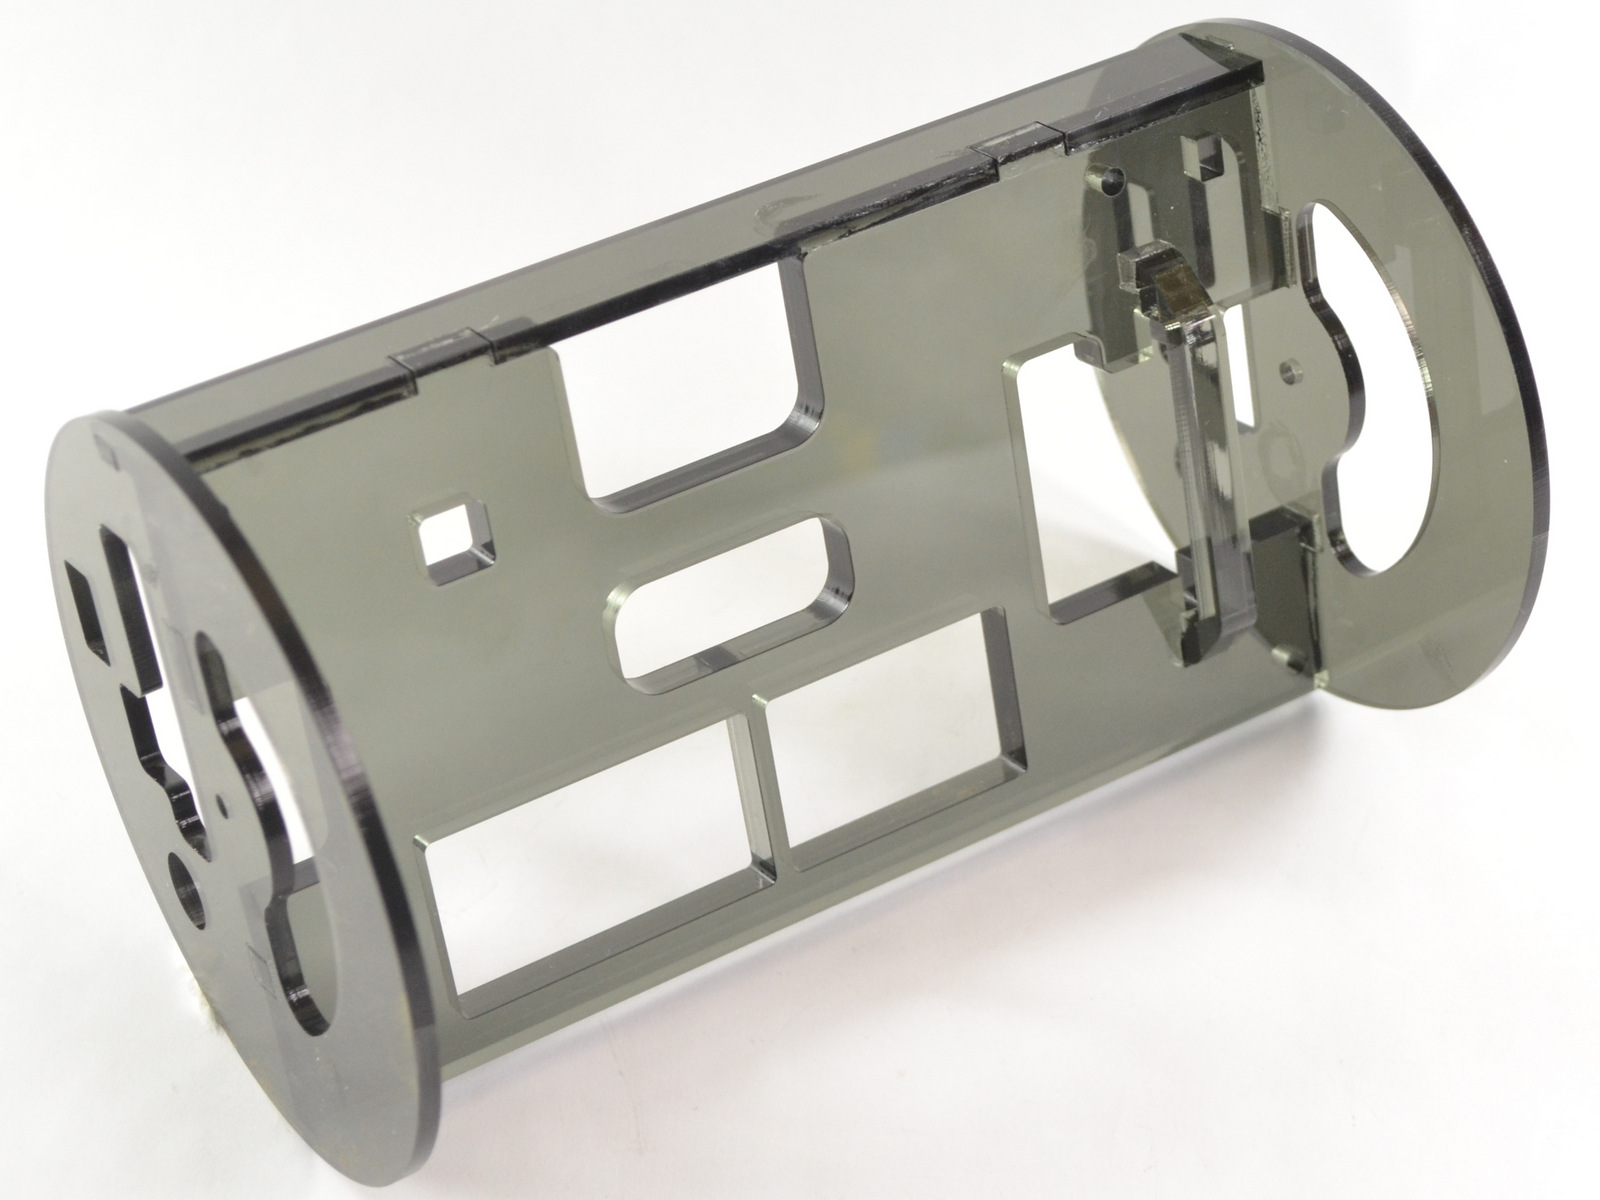
\includegraphics[width=6cm,height=5cm]{img/cap3/3_3/chasis_electronico}}
  \end{center}
  \caption{Soporte de la cámara y electrónica}
  \label{fig:ROV-chasis}
\end{figure}

\subsection{Tapas del chásis}
\label{subsec:tapasChasis}

Al igual  que en el punto anterior, antes de comenzar con el montaje de la tapa, se necesitarán ciertas herramientas para el correcto ensamblaje.

Las herramientas necesarias son: guantes, gafas, cúter, cemento acrílico,  SuperGlue y epoxy (epoxy es un tipo de pegamento que soporta estar en contacto con el agua). Una vez hayamos obtenido todos los materiales empezaremos con el montaje.

En este caso, existen dos tapas. En la primera (la superior), necesitaremos una jeringa proporcionada por la comunidad de OpenROV, la cual utilizaremos para preparar la impermeabilización y el sellado de los componentes software del robot.

En la segunda tapa, está el conector DB-25, el cual, conecta todos los componentes eléctricos a la placa del controlador. Una vez realizado el montaje de la tapa, se pegará en el espacio sobrante el conector DB-25 y se colocarán los cables adecuadamente en el hueco de la tapa. Cuando esté todo debidamente colocado se pegará la tapa superior al montaje realizado, lo cual dejará todo debidamente sellado. Este hueco, se rellenará con el epoxy para que no entre agua por la ranura.

\begin{figure}[hbtp]
  \begin{center}
    \subfigure[Tapa inferior desmontada]{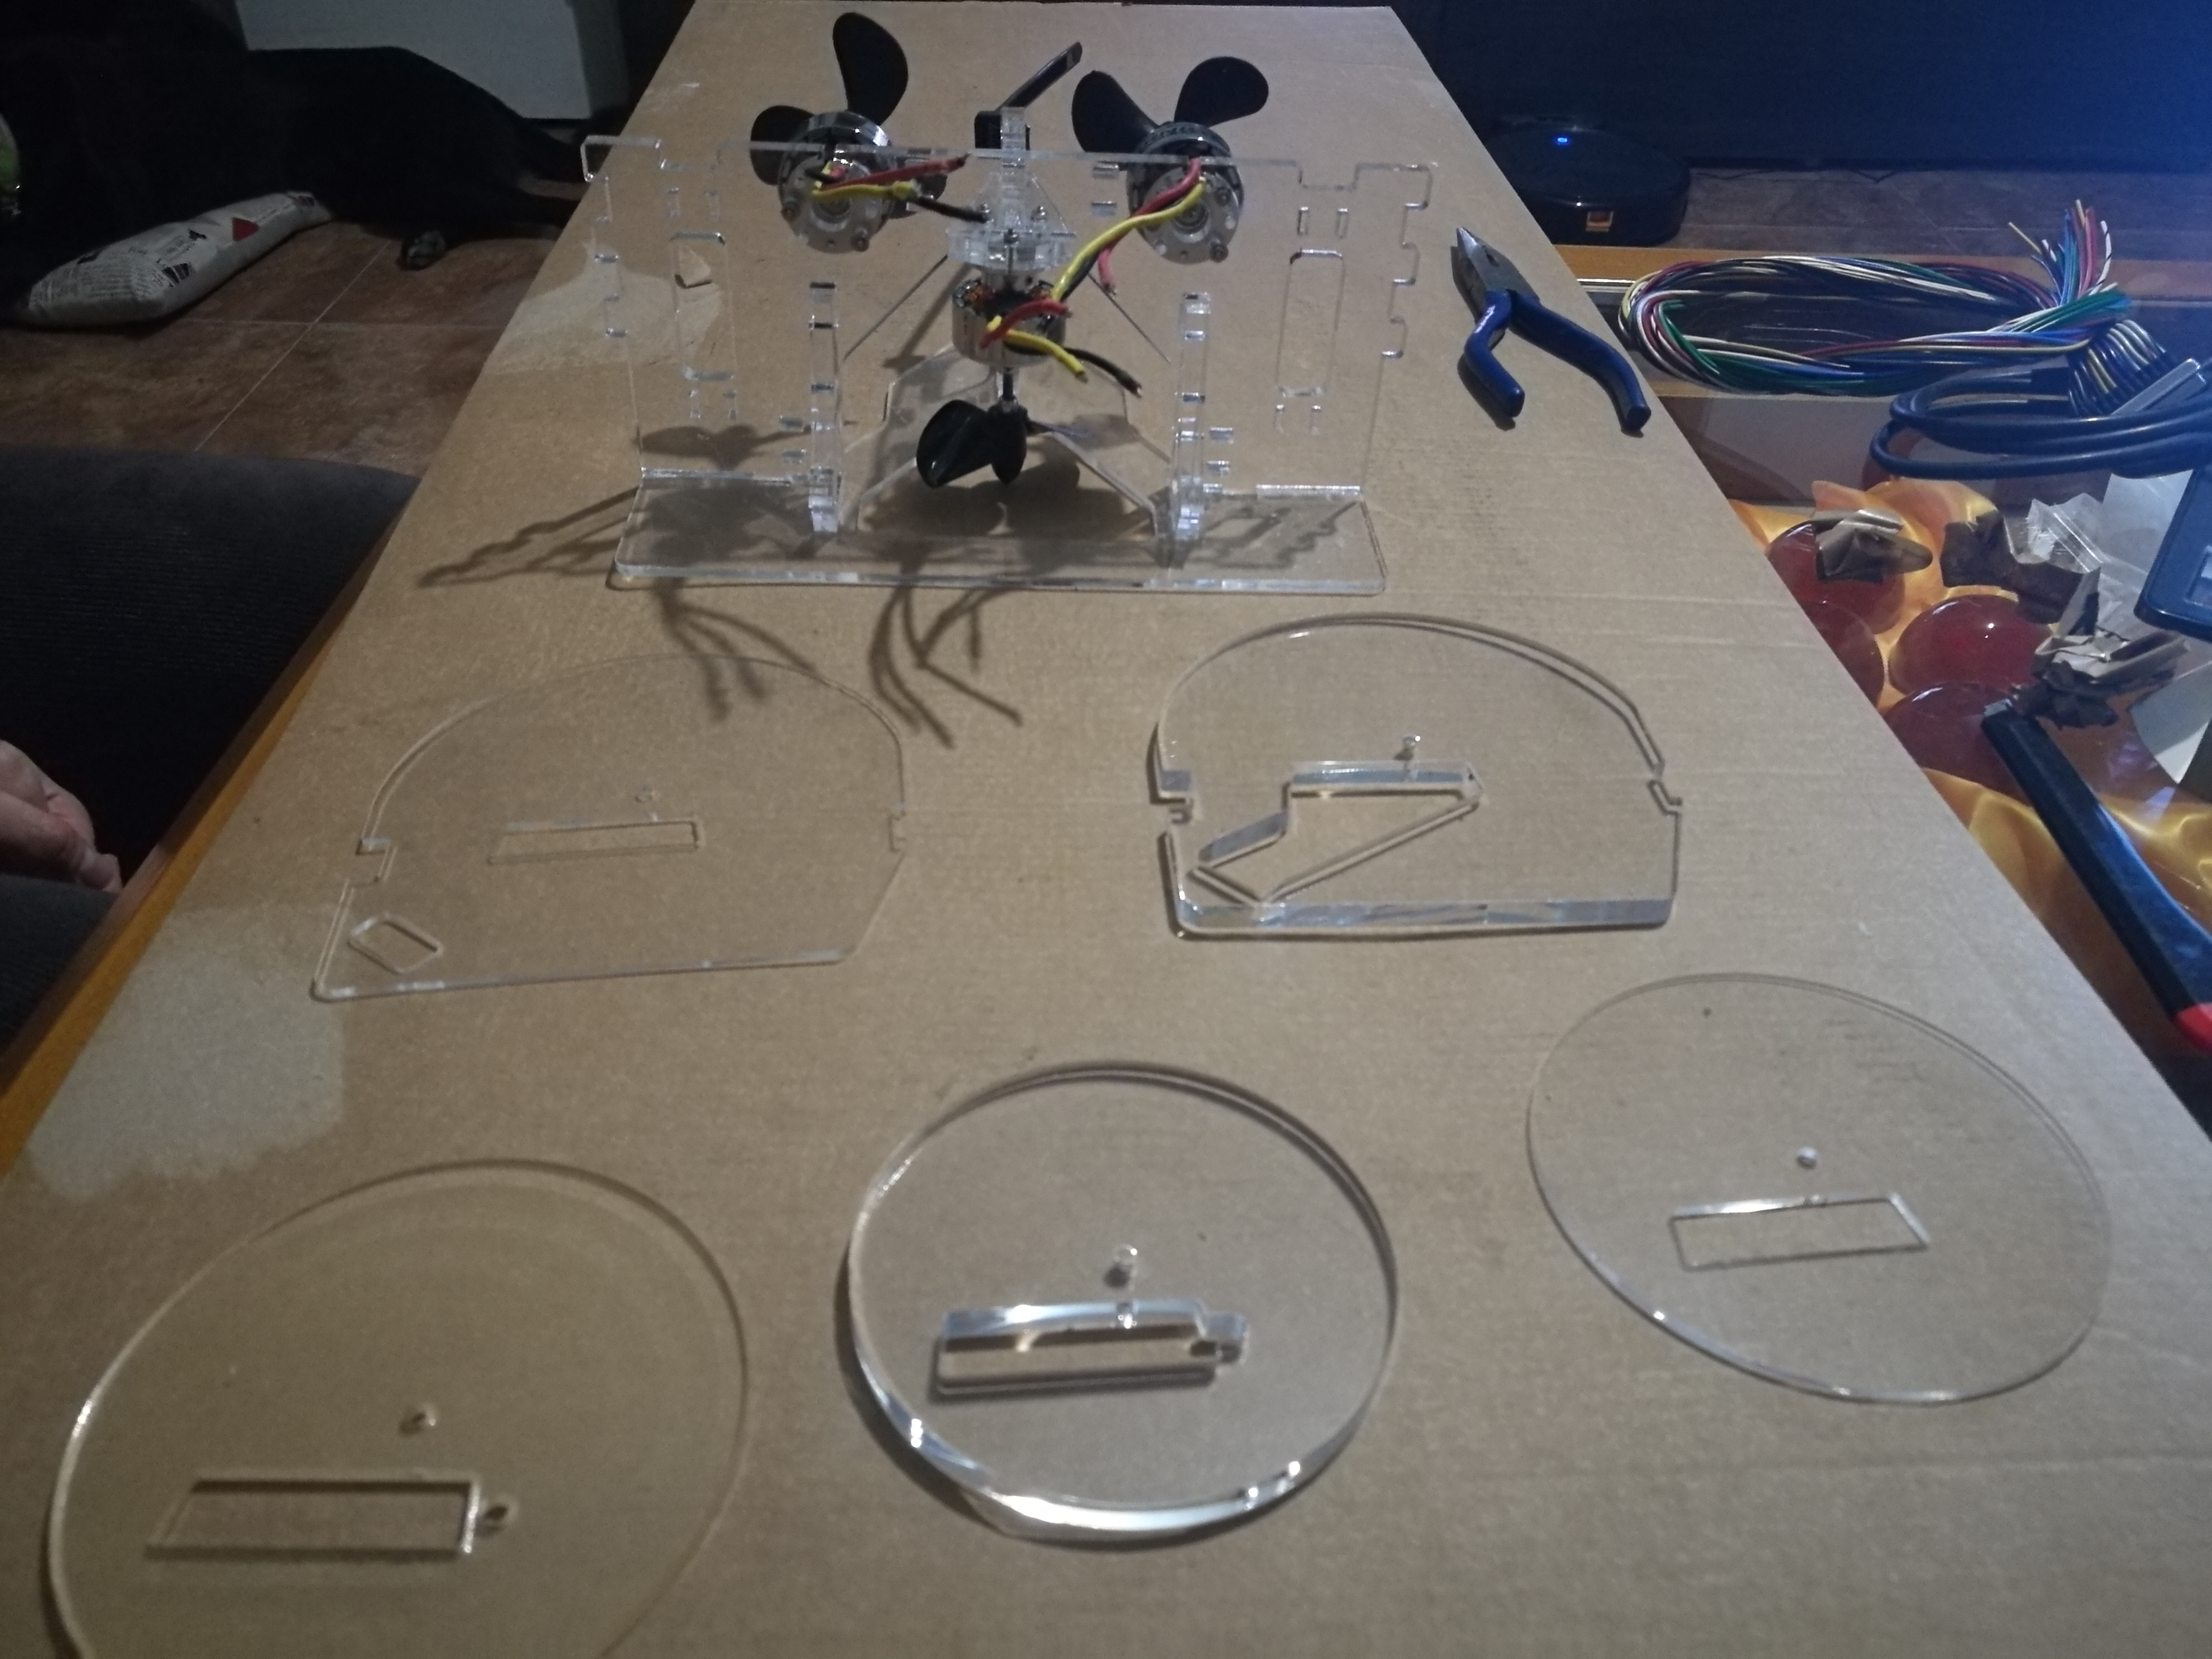
\includegraphics[width=6cm,height=5cm]{img/cap3/3_3/tapa_inf_desmontada}}
    \subfigure[Tapa inferior montada]{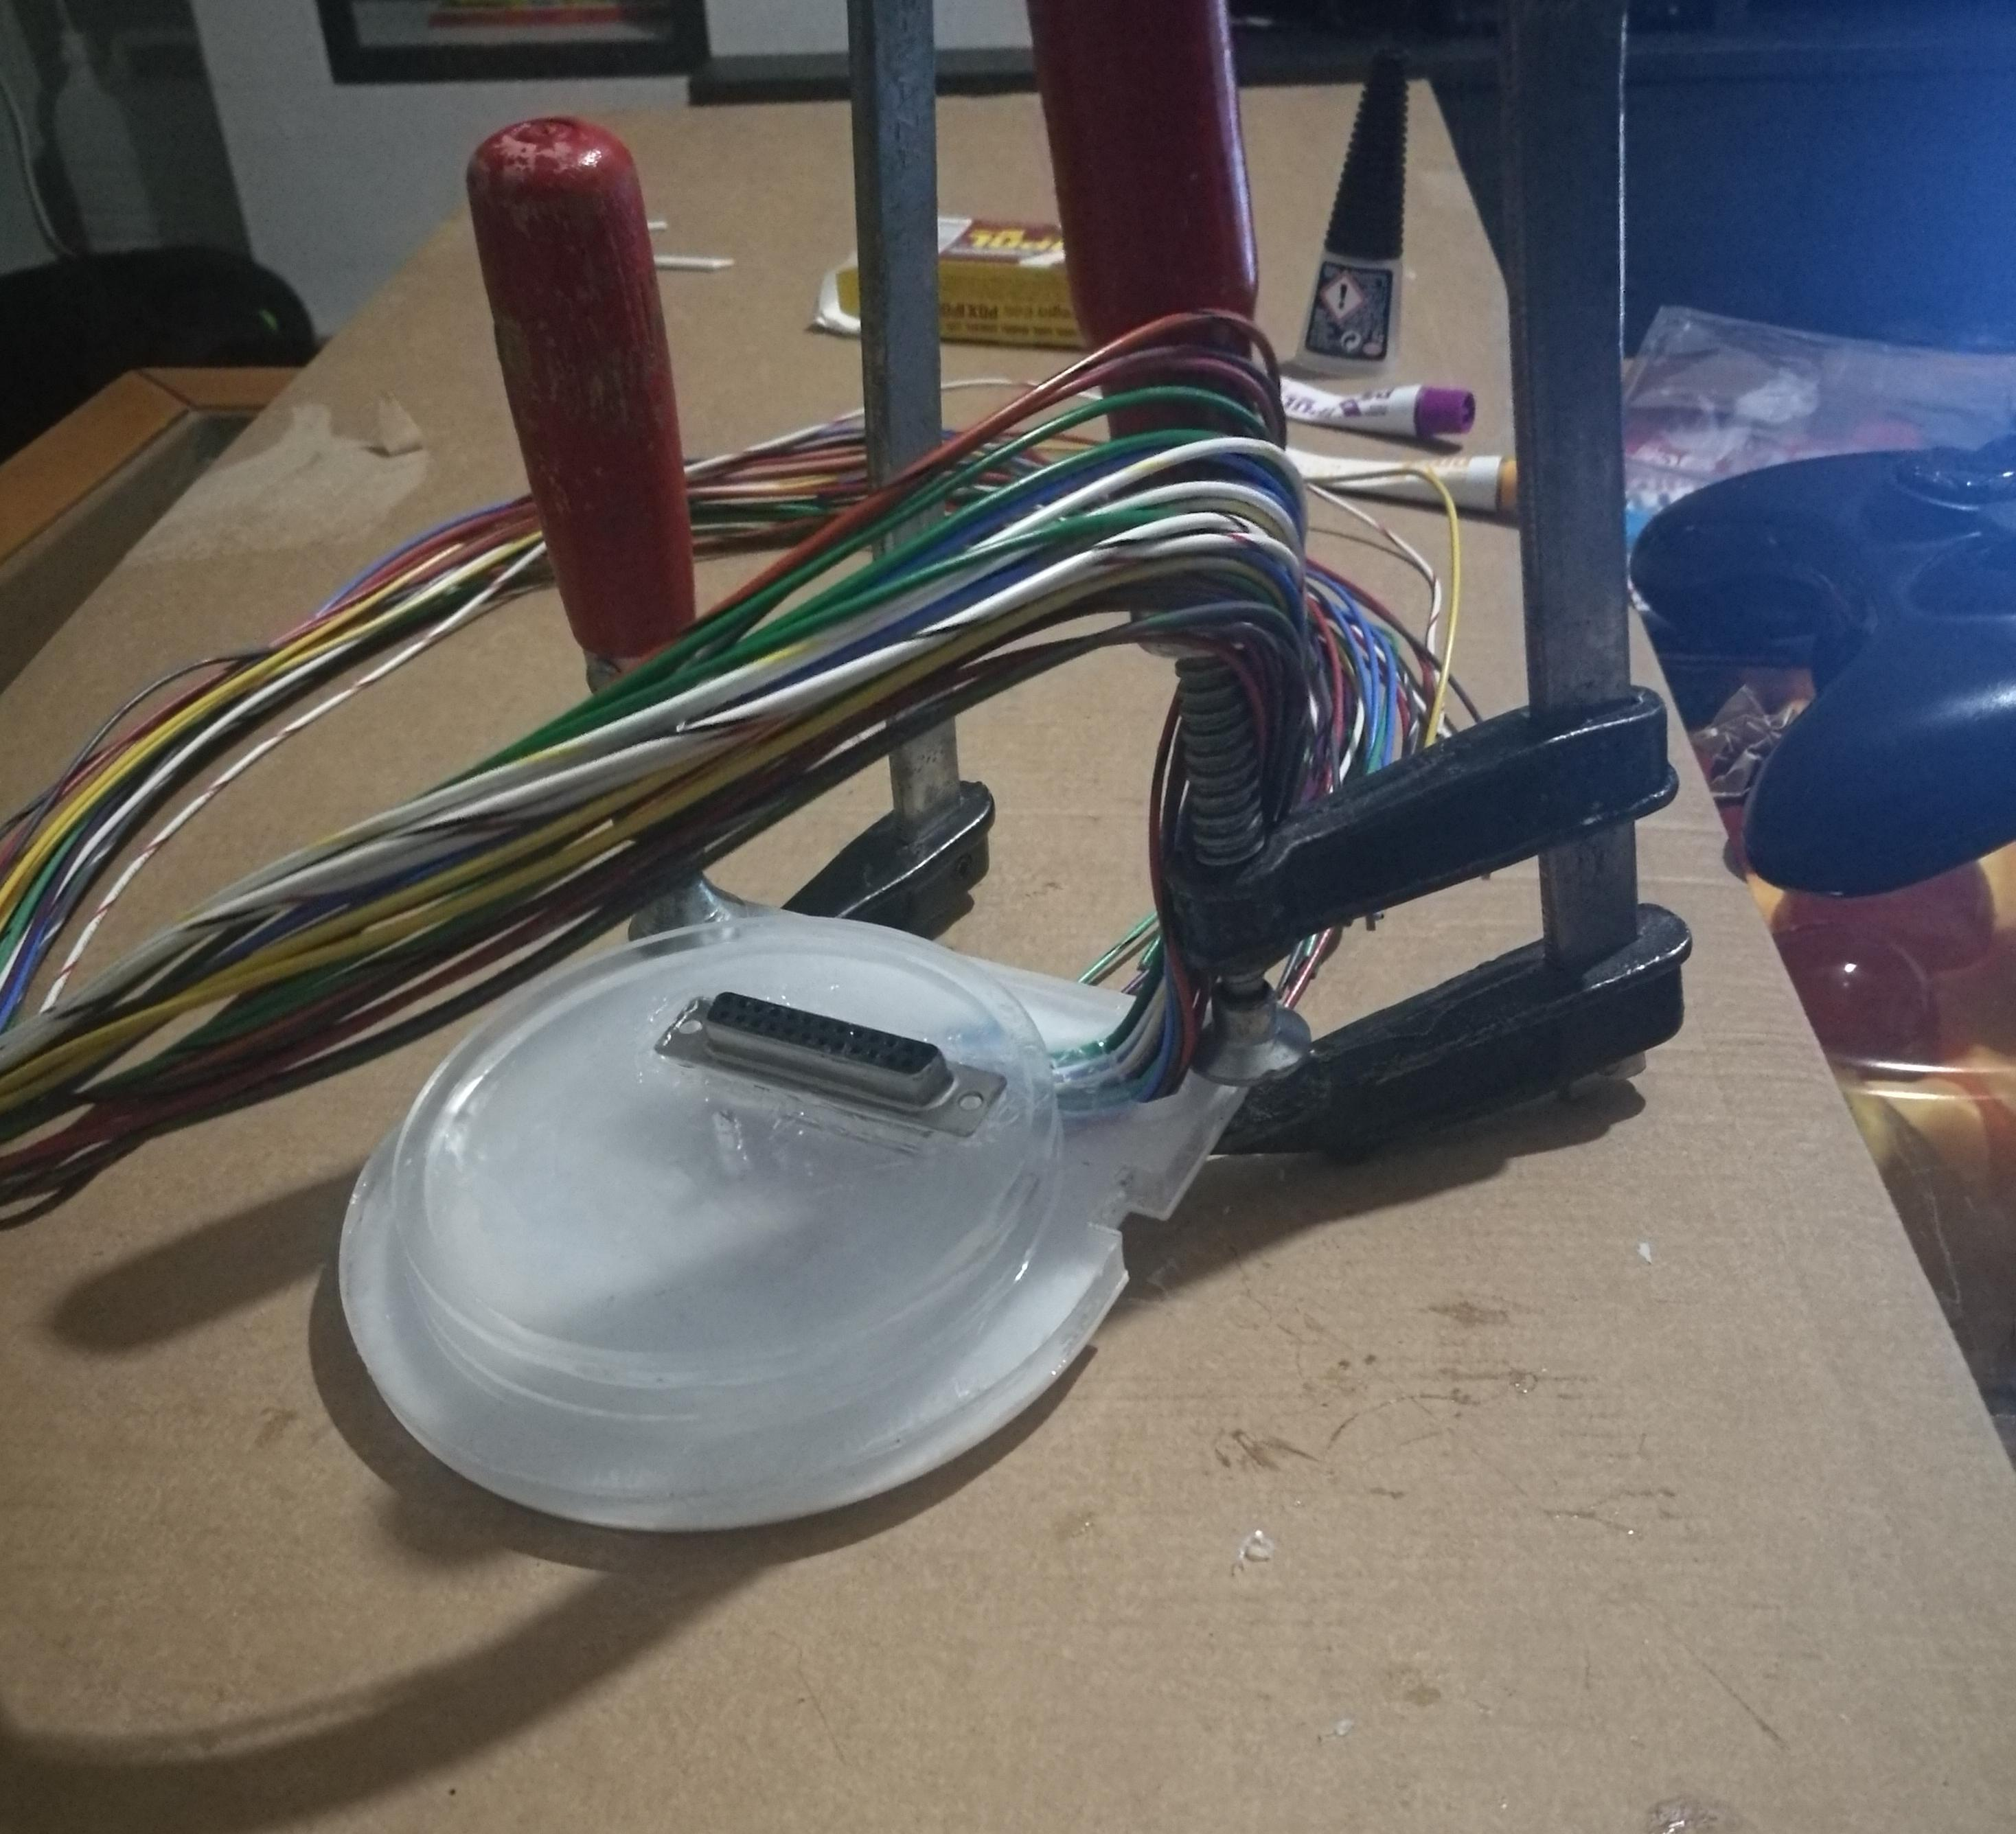
\includegraphics[width=6cm,height=5cm]{img/cap3/3_3/tapa_inf}}
  \end{center}
  \caption{Tapa inferior}
  \label{fig:tapa_iferior}
\end{figure}

\subsection{Electrónica}
\label{subsec:electronica}

Este es el punto crucial del funcionamiento del robot y se necesita especial atención en cada uno de los pasos. 

Al igual que en los apartados anteriores, necesitaremos material especial, entre los que están el soldador, estaño, PLC, BeagleBone, tijeras y destornilladores.

Para empezar, desmontaremos los PLC para sacar el hardware, el cual utilizaremos más adelante.
Uno de los PLC estará interno en el robot, y el otro, será el extremo conector que comunicará el ROV con el portátil.

Continuaremos con el BeagleBone Black (BBB), el cual, es el procesador principal en el ROV. Funciona junto con un Ardunio en el tablero del controlador para controlar las muchas funciones del ROV.

El cable USB del BeagleBone lo utilizaremos más adelante.

Una vez juntos el PLC, el BeagleBone y la placa del ROV, uniremos estos tres elementos para formar el hardware del robot. Se conectará primero la placa del ROV, en la que el conector RJ-45 irá conectado al hardware PLC. Una vez realizada esa conexión, procederemos a implantar en las ranuras el BeagleBone, y atornillaremos para obtener una mejor sujeción.

\begin{figure} [hbtp]
  \begin{center}
    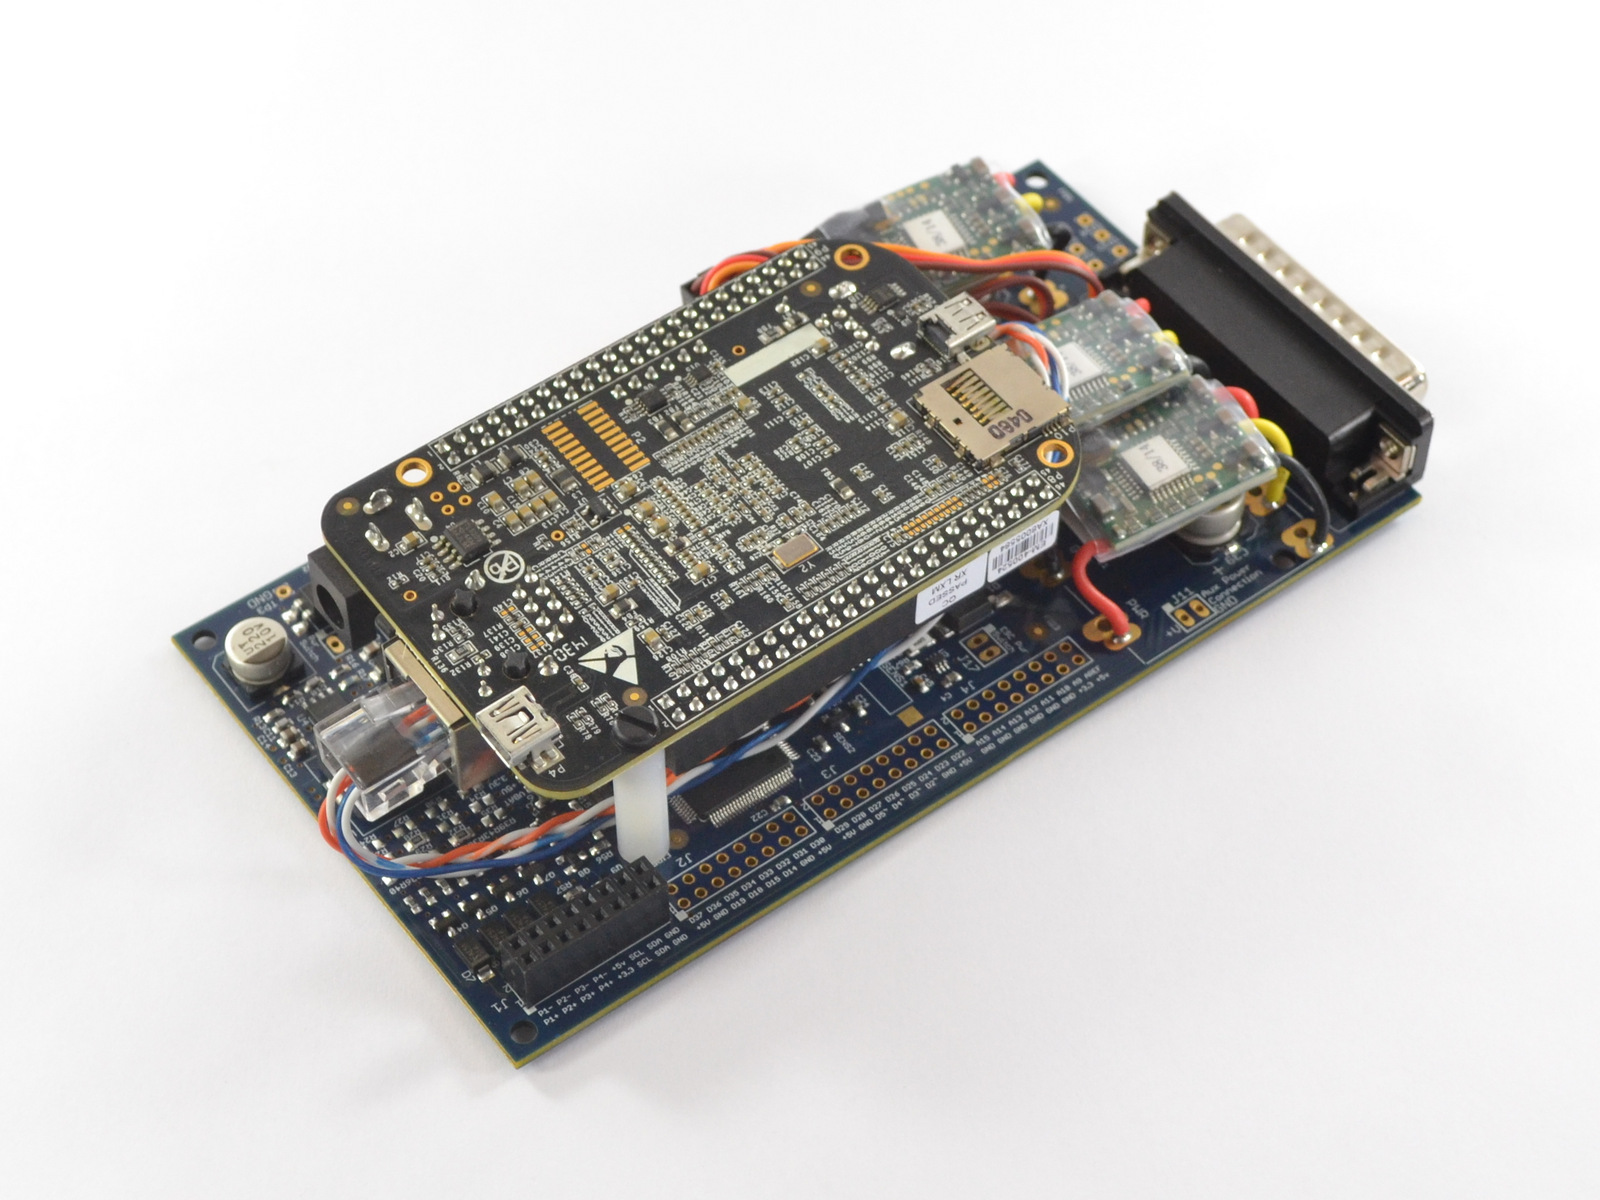
\includegraphics[width=8cm]{img/cap3/3_3/electronica}
  \end{center}
  \caption{Raspberry Pi + PLC + BeagleBone}
  \label{fig:electronica}
\end{figure}

Después, conectaremos el servo al chasis, el cual va a servir para mover la cámara verticalmente. Hay que asegurarse de que quede centrado.

Continuaremos con la soldadura de los láser y unos cables a la placa de video del ROV.

\begin{figure} [hbtp]
  \begin{center}
    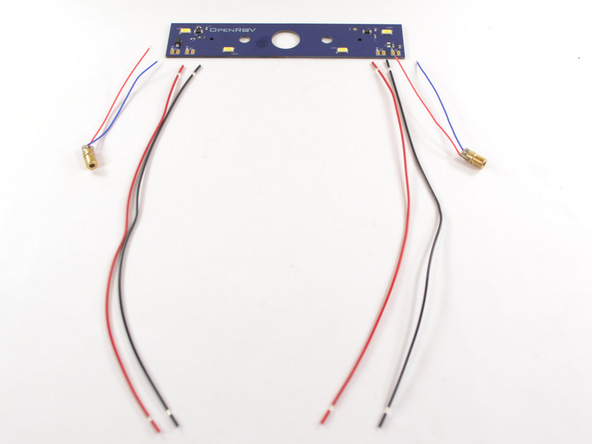
\includegraphics[width=8cm]{img/cap3/3_3/electronica_camara}
  \end{center}
  \caption{Electrónica de la cámara}
  \label{fig:electronica_camara}
\end{figure}

Cuando estén debidamente soldados, se colocará el chasis de la cámara, junto con lo que acabamos de soldar y la cámara. A estos tres elementos los juntaremos con tornillos y tuercas. Para finalizar con este paso, comprobamos que hay un conector al cual enchufaremos un cable que irá directo a la placa principal del ROV.

Para la sujeción de la cámara utilizaremos el chasis principal, al que atornillaremos para fijar la cámara. En la parte izquierda del chasis principal, existe un hueco en el que irá el motor servo, el cual ha sido modificado para esa ubicación, eliminándole una de las astas para que se quede fijo en una posición y pueda mover la cámara en el eje vertical.

Para finalizar este apartado, se conectará el hardware del robot en el lado opuesto de la cámara, y se fijará con tornillos. Se realizará la conexión de los cables a sus ranuras correspondientes.

\subsection{Enrutamiento}
\label{subsec:enrutamiento}

En esta fase, se va a requerir unas herramientas más específicas para realizar el montaje, ya que necesitaremos soldar e impermeabilizar con una pistola de calor, además, de tijeras, epoxy, super Glue y bridas.

Empezaremos calculando la distancia de los cables y separaremos los de color verde claro y naranja, para la conexión de las baterías. Los cables verdes oscuros, rojos y azules, los utilizaremos para el montaje de los servomotores. Iremos fijando los cables con las bridas para una correcta colocación.

Cada uno de los tres motores servo, lleva tres cables, los cuales soldaremos con los cables correspondientes. Una vez soldados, con una silicona especial se rellenará el espacio del cable soldado y con la pistola de calor se fijará e impermeabilizará.

\begin{figure} [hbtp]
  \begin{center}
    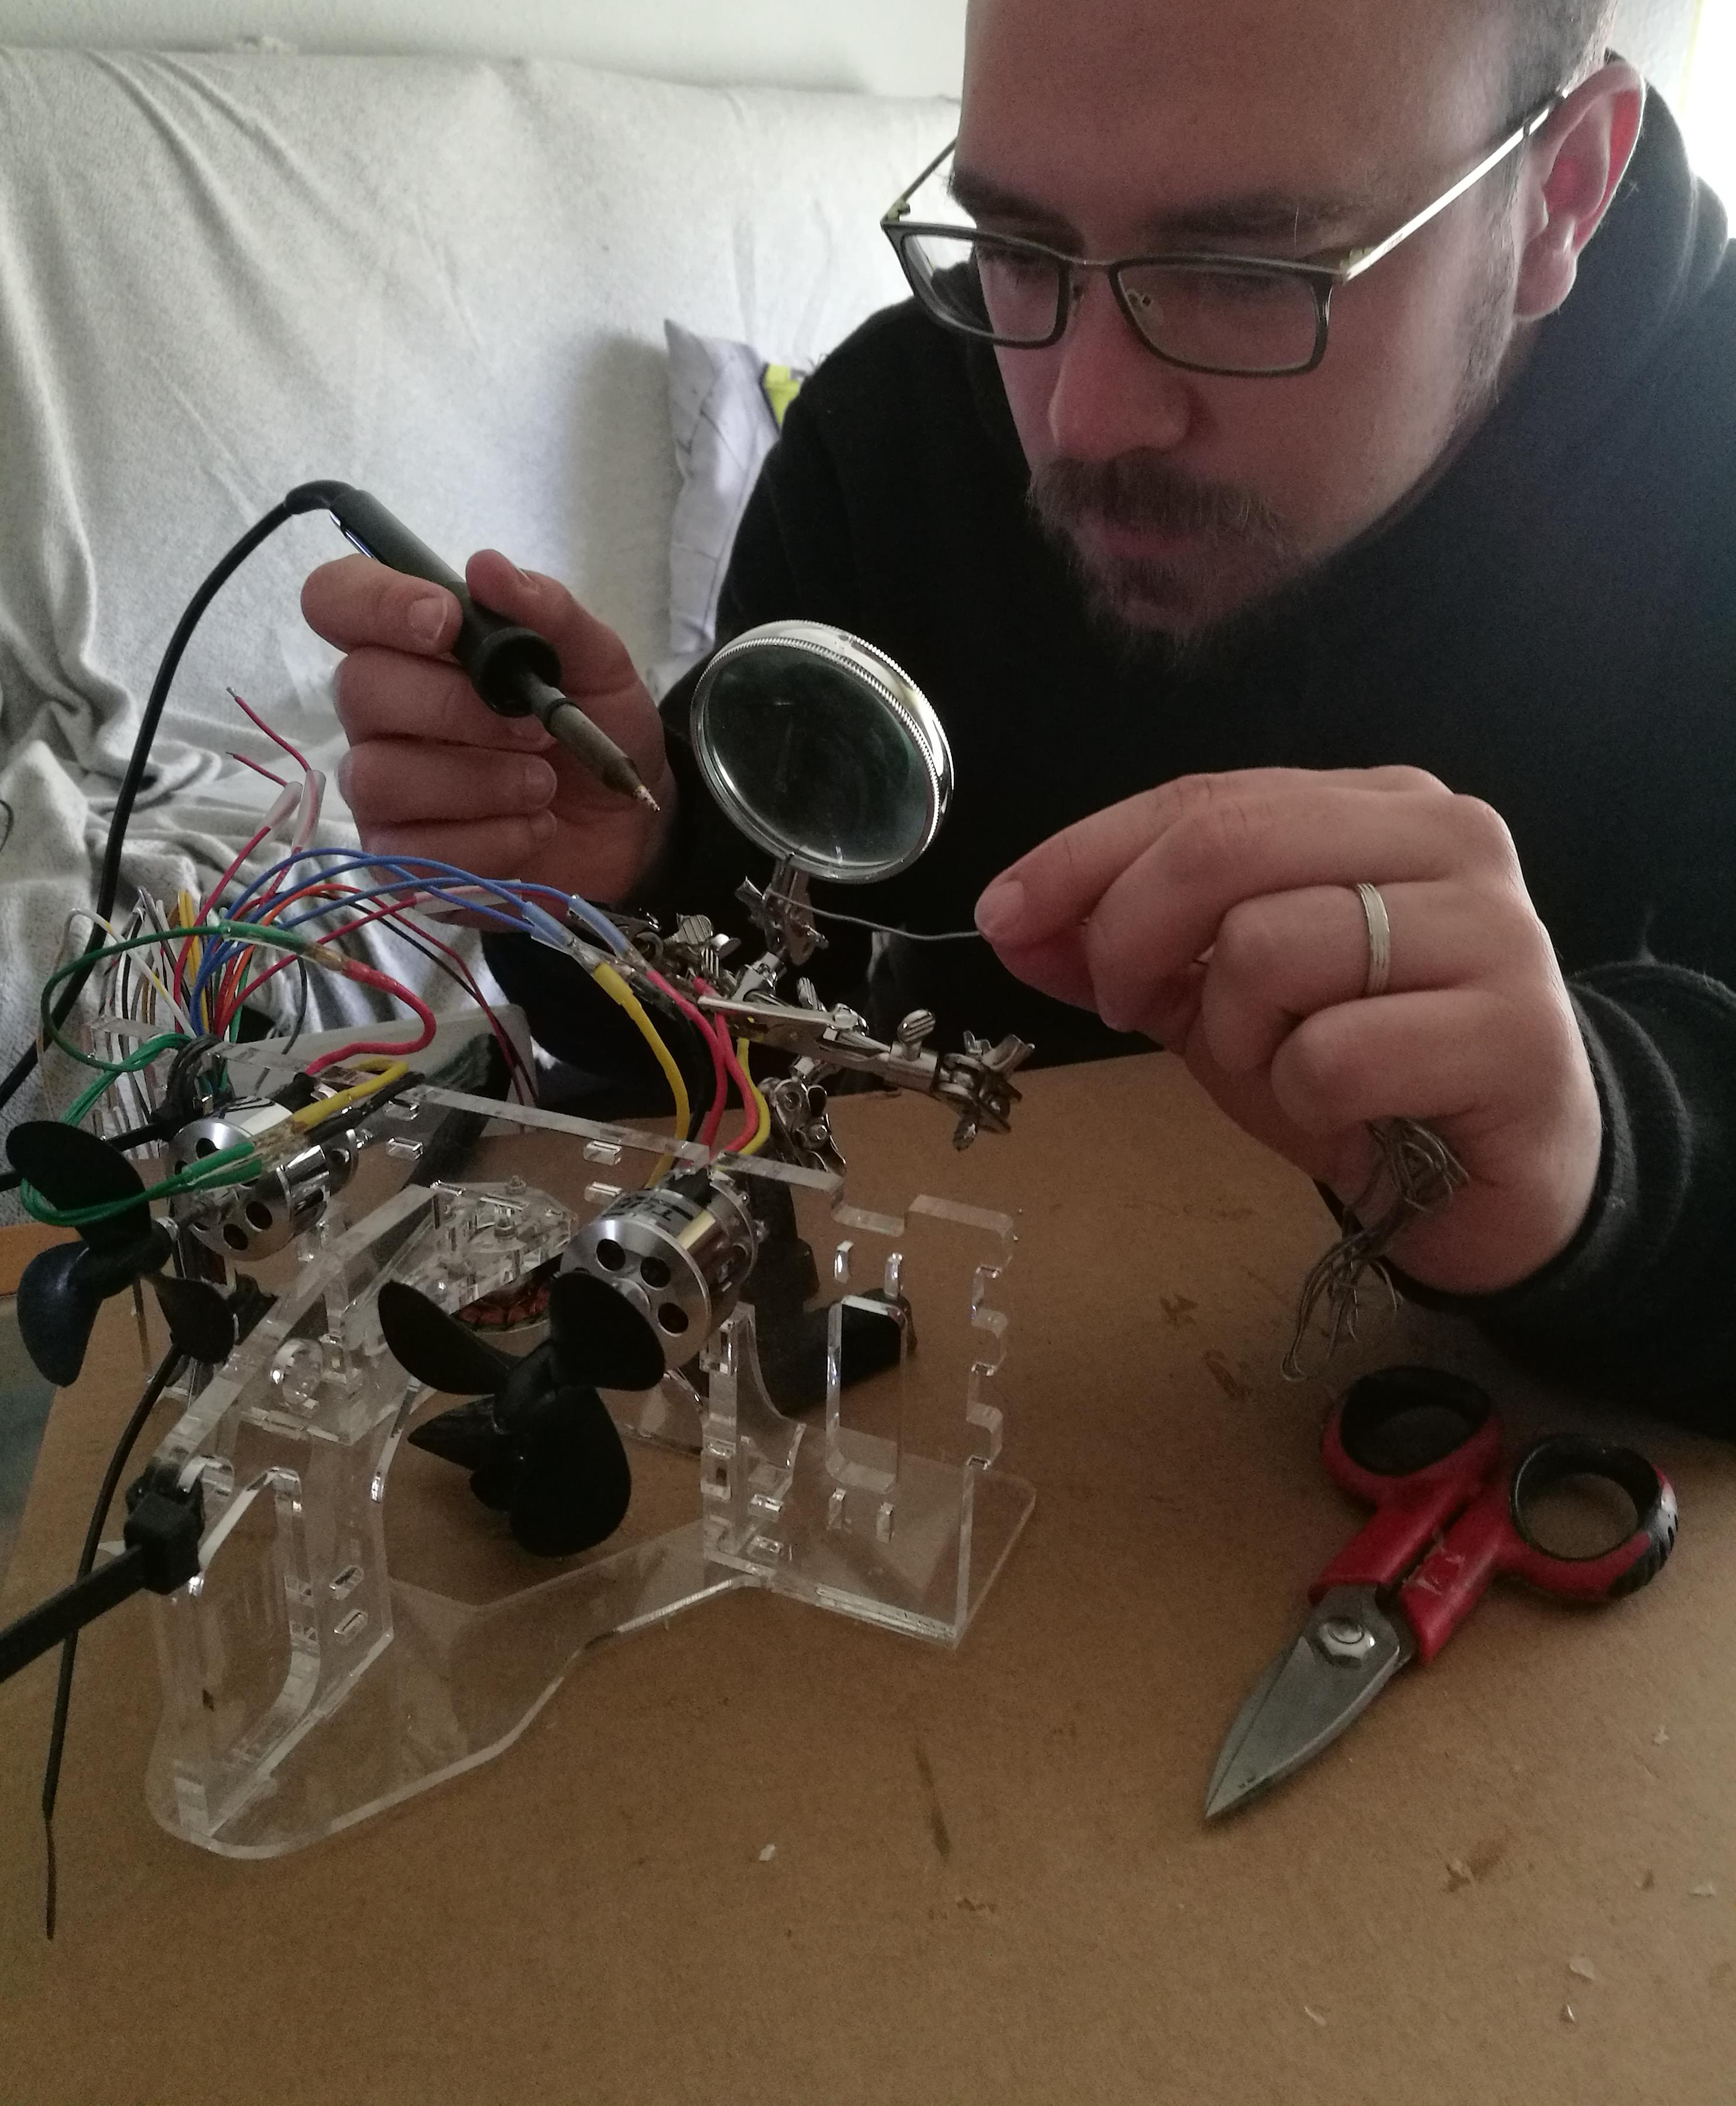
\includegraphics[width=8cm]{img/cap3/3_3/soldar}
  \end{center}
  \caption{Soldadura de cables}
  \label{fig:soldar}
\end{figure}

Los diez cables sobrantes se sellarán, ya que servirían para sensores y luces extra que no  utilizaremos en este proyecto.

Continuaremos con el montaje de los dos tubos de la batería. Primero, necesitaremos realizar el montaje de las piezas y soldaremos el muelle (borne) con un chip facilitado por la comunidad de ROV. Esta parte irá con el polo negativo de las baterías.
En el extremo del cable sobrante, se rellenará el terminal con estaño y se soldará al cable formando la parte positiva en la que se conectará la batería.

\subsection{Final}
\label{subsec:final}

En la parte final del montaje, será necesaria una soldadura con el cable de par trenzado que es el encargado de mandar la señal al portátil.

Para asegurar esa soldadura, utilizaremos una brida de un tamaño mayor a las usadas anteriormente, y soldaremos un cable preservado en el apartado anterior con el par trenzado.

Este cable de par trenzado mide cien metros, el cual, en el extremo opuesto al ROV, irá conectado al PLC. Gracias a este cable, el robot se podrá sumergir a una distancia de cien metros. Por eso, y para mayor seguridad, usaremos la brida, enroscaremos el cable en ella y lo finalizaremos recubriéndolo con cinta adhesiva.
En el cuerpo principal del ROV, sujetaremos con unas gomas los tubos que llevarán las baterías, y lo fijaremos en los extremos con dos varillas de metal.

Aislaremos el hardware con un tubo cilíndrico trasparente de polimetilmetacrilato, pero antes de fijarlo, limaremos los extremos del cilindro para una mejor conexión con las tapas.

Cuando todo el montaje esté terminado, pondremos más seguridad al hardware, añadiendo una cuerda que hará presión.

Además, colocaremos dos pesas de trescientos gramos en los brazos del ROV para que la sumersión sea más fácil y fiable.

\section{Conectividad OpenROV}
\label{cap:Conectividad OpenROV}
  
\subsection{Diseño de Conectividad}
\label{subsec:disenio}

Para encender el ROV, necesitaremos el cable mini USB y el cable ethernet debidamente colocado en el extremo del PLC y estos a su vez al portátil.

\begin{figure} [hbtp]
\begin{center}
  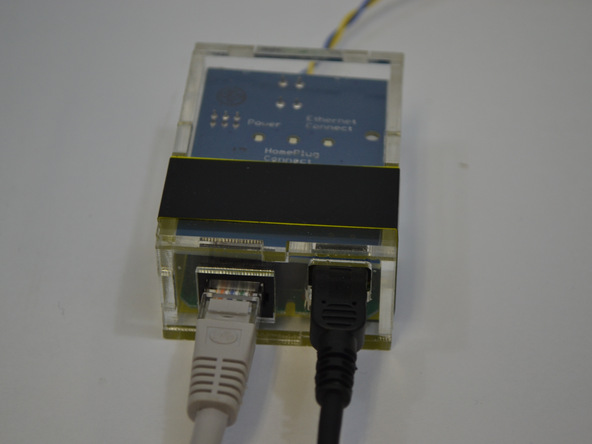
\includegraphics[width=8cm]{img/cap3/3_4/plc_externo}
\end{center}
\caption{PLC externo}
\label{fig:plc_ext}
\end{figure}
  
El conector USB actúa como el interruptor de encendido/apagado para el ROV.

El ROV tiene una dirección IP estática incorporada de 192.168.254.1, por lo que para conectarse con ella, la dirección IP de ethernet de su computadora debe estar en la misma subred, es decir, 192.168.254.2. La máscara de subred debe establecerse en 255.255.255.0.

Pero para poder mostrar la página, antes debemos realizar una serie de pasos, en la que necesitaremos una microSD para realizar la configuración del ROV.
  
\begin{itemize}
\item El primer paso, es descargar la imagen más reciente de OpenROV (30.0.3), una vez descargado, se descomprime el archivo .zip, dejando en el directorio de descarga el fichero .img.
\item Para cerciorarse de que la mircoSD esta vacía, se formatea con el programa SDFormatter, luego, con el programa Win32DiskImager, escribiremos en la tarjeta microSD el fichero .img, esperamos alrededor de 5 minutos a que se complete la escritura. Cuando haya terminado, removemos la tarjeta microSD del portátil.
\item Conectamos  la tarjeta microSD a el Beagle Bone, y conectamos el ROV con el cable USB para encenderlo. Los LED de Usuario de la placa Beagle Bone parpadearán para mostrar que laa imagen se está aplicando a la memoria de dicha placa. El proceso dura aproximadamente 15 minutos, en ese tiempo, los cuatro led deben estar encendidos, de no ser así, habría que repetir este punto nuevamente.

Cuando esté completo, retiraremos el cable USB del portátil para desconectar el ROV y retiraremos la tarjeta microSD de la placa Beagle Bone.

Terminado este proceso, volveremos a conectar la tarjeta en el portátil.

\begin{figure} [hbtp]
\begin{center}
  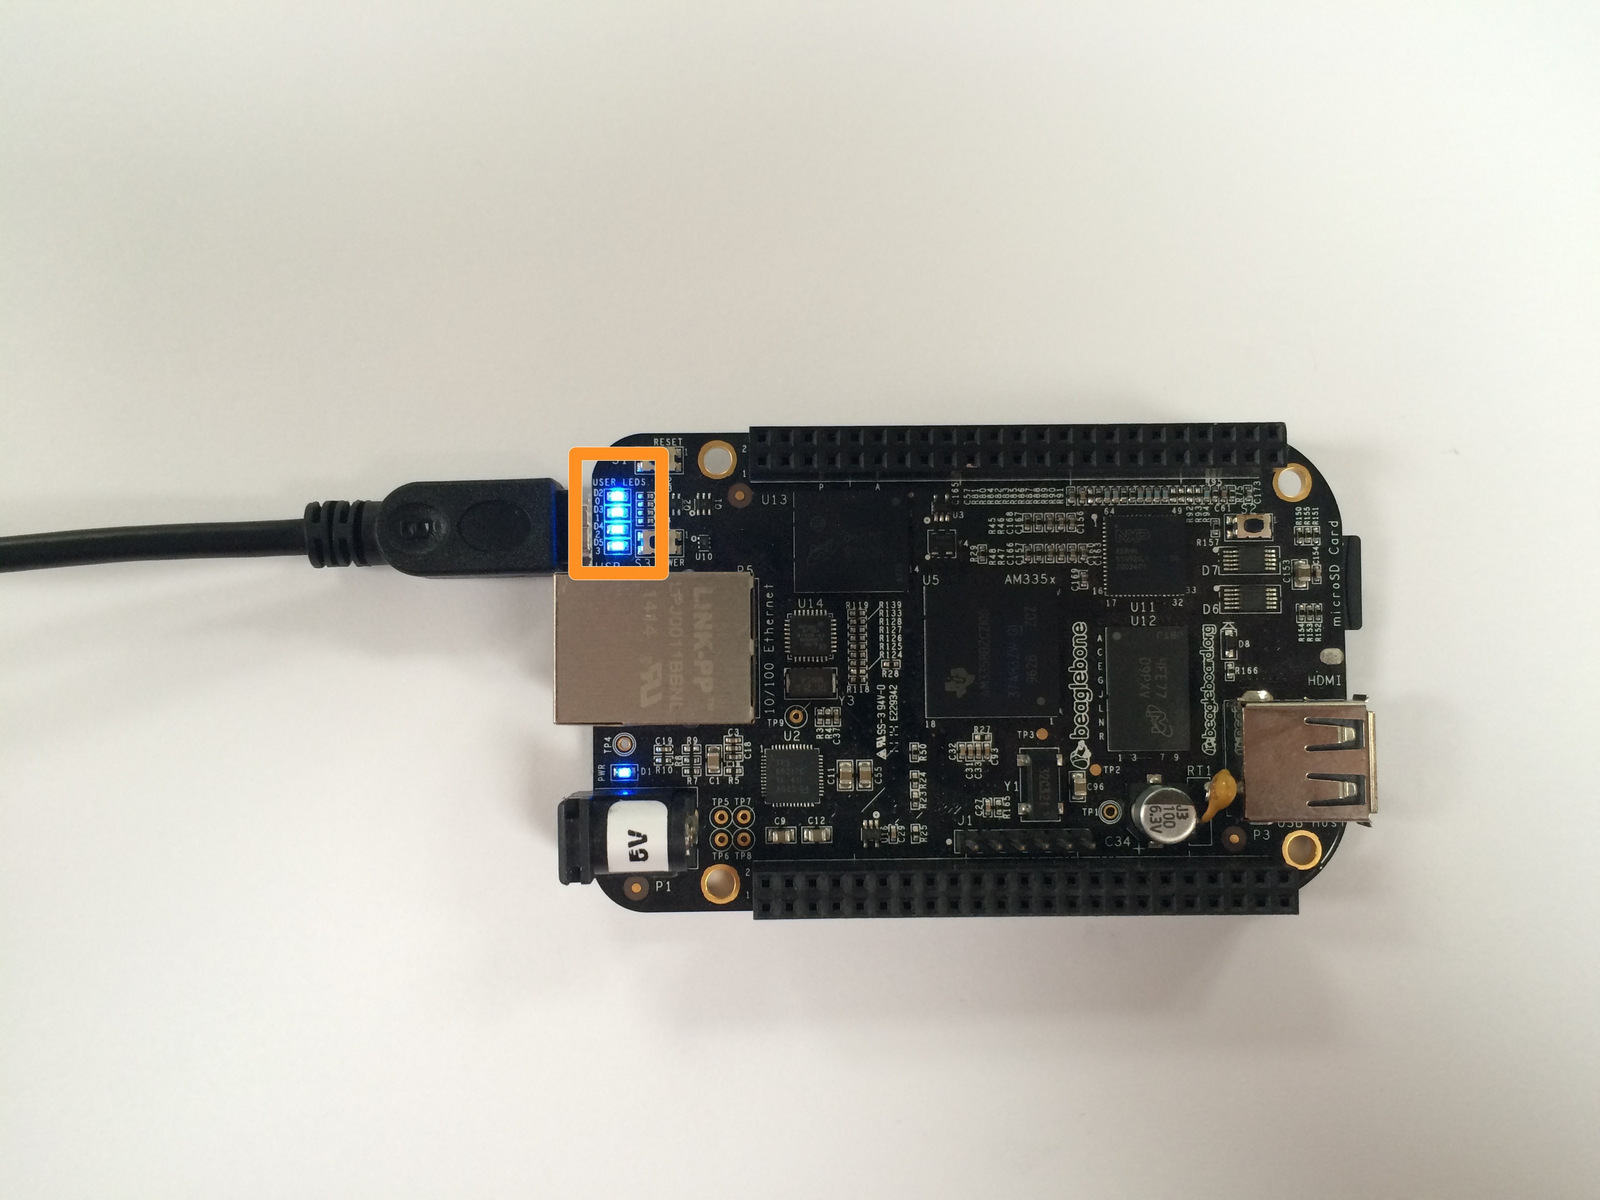
\includegraphics[width=8cm]{img/cap3/3_4/BBB}
\end{center}
\caption{BeagleBone configurada}
\label{fig:bbb}
\end{figure}
\item Como se mencionó al principio del apartado, el ROV tiene una dirección IP estática incorporada de 192.168.254.1, por lo que para conectarse con ella, el ordenador debe tener una dirección similar pero con el último número configurado  distinto de 1, por ejemplo, podemos usar la dirección "192.168.254.2". La máscara de subred debe establecerse en 255.255.255.0.

En Windows 8 la configuración sería:

\renewcommand{\lstlistingname}{Configuración}
\begin{lstlisting}[caption= Windows 8, label={lst:config_w8}]
Ir  al Panel de control.
Seleccionar Red e Internet.
Red y centro compartido → (click) cambiar configuración de adaptador → (click) ethernet.
Propiedades →(click) usar la siguiente dirección IP
Insertarla dirección IP 192.168.254.2
\end{lstlisting}

\begin{figure} [hbtp]
\begin{center}
  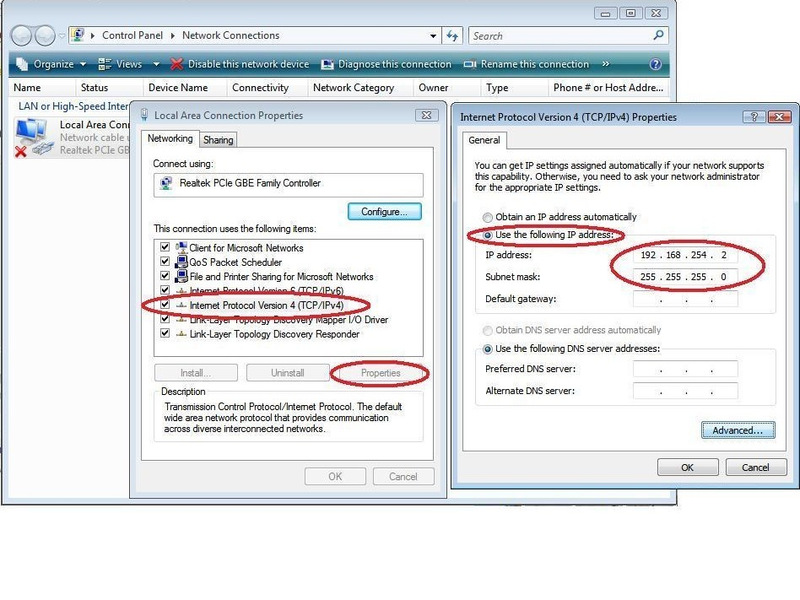
\includegraphics[width=8cm]{img/cap3/3_4/conexion}
\end{center}
\caption{Conexión Windows 8}
\label{fig:w8}
\end{figure}

En Ubuntu la configuración de una nueva IP estática:

\renewcommand{\lstlistingname}{Configuración}
\begin{lstlisting}[caption= Ubuntu, label={lst:config_ubuntu}]
  # Abrir el terminal (Ctrl + Atl + T).
  # Comprobamos las interfaces del equipo:  
  $ ifconfig -a
  # Editamos el archivo de configuracion de las interfaces:  
  $ sudo vim /etc/network/interfaces

  # Configuracion de direccion IP fija para el interfaz eth0
    auto eth0
    iface eth0 inet static
    address 192.168.254.2
    netmask 255.255.255.0
    network 192.168.254.0
    broadcast 192.168.254.255
    gateway 192.168.254.1
\end{lstlisting}

  Donde:
    \subsubitem address es la dirección IP que quieres ponerle a tu máquina.
    \subsubitem netmask es la máscara de subred de esa dirección IP.
    \subsubitem network es la red a la que pertenece esa dirección IP.
    \subsubitem broadcast es la direción IP de difusión de esa red.
    \subsubitem gateway es la dirección IP de la puerta de enlace predeterminada.

\subitem Reiniciamos las interfaces de red para aplicar los cambios:

\renewcommand{\lstlistingname}{}
\begin{lstlisting}[caption=Reinicio, label={lst:reset}]
  $ sudo /etc/init.d/networking restart
\end{lstlisting}
\item Abriremos el navegador Google-Chrome, y en la barra de direcciones escribiremos la IP 192.168.254.1:8080, que es la dirección IP de OpenROV. Presionaremos <enter> y en un periodo de aproximadamente 20 segundos aparecerá la interfaz de OpenROV.
\item Para finalizar, deberemos actualizar el firmware, en la web, presionaremos el botón de configuración en la parte superior derecha de la pantalla y presionaremos “Cargar firmware desde la tarjeta SD a Ardruino”
La tarjeta no microSD no debe estar en el ROV, presionaremos “Mostrar Detalles” y seguidamente, “Aplicar nuevo Firmware”.
El proceso dura aproximadamente entre 5-10 minutos.
Una vez que la carga sea exitosa, se desconectará el cable USB del portátil para apagar el ROV, para realizar el reinicio, volveremos a conectar el cable USB al portátil.


\begin{figure} [hbtp]
\begin{center}
  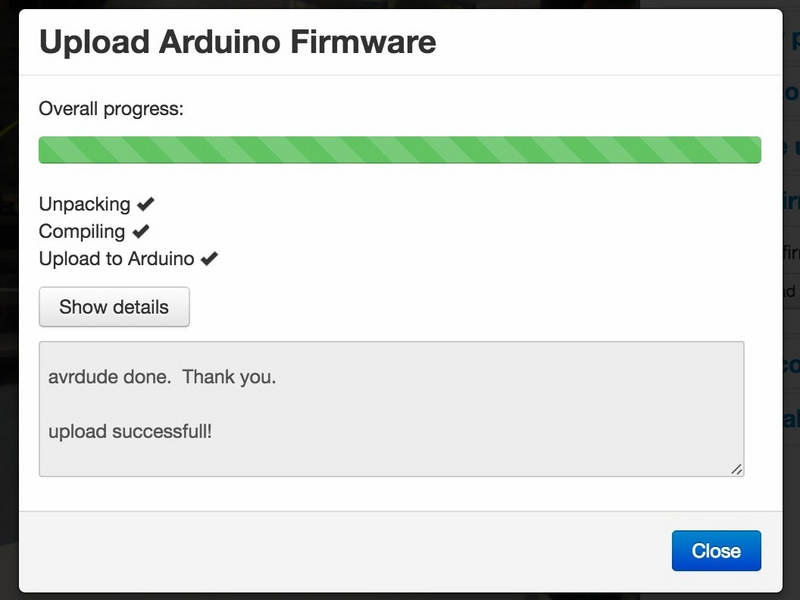
\includegraphics[width=8cm]{img/cap3/3_4/firmware}
\end{center}
\caption{Actualización firmware}
\label{fig:firmware}
\end{figure}

\end{itemize}
  
  
  
\subsection{Puesta a punto de los elementos}
\label{subsec:elementos}
  \subsubsection{Cámara}
  \label{subsubsec:camara}
Ajustaremos el foco de la lente de la cámara hasta que la imagen pueda verse con total nitidez.
\begin{figure} [hbtp]
\begin{center}
  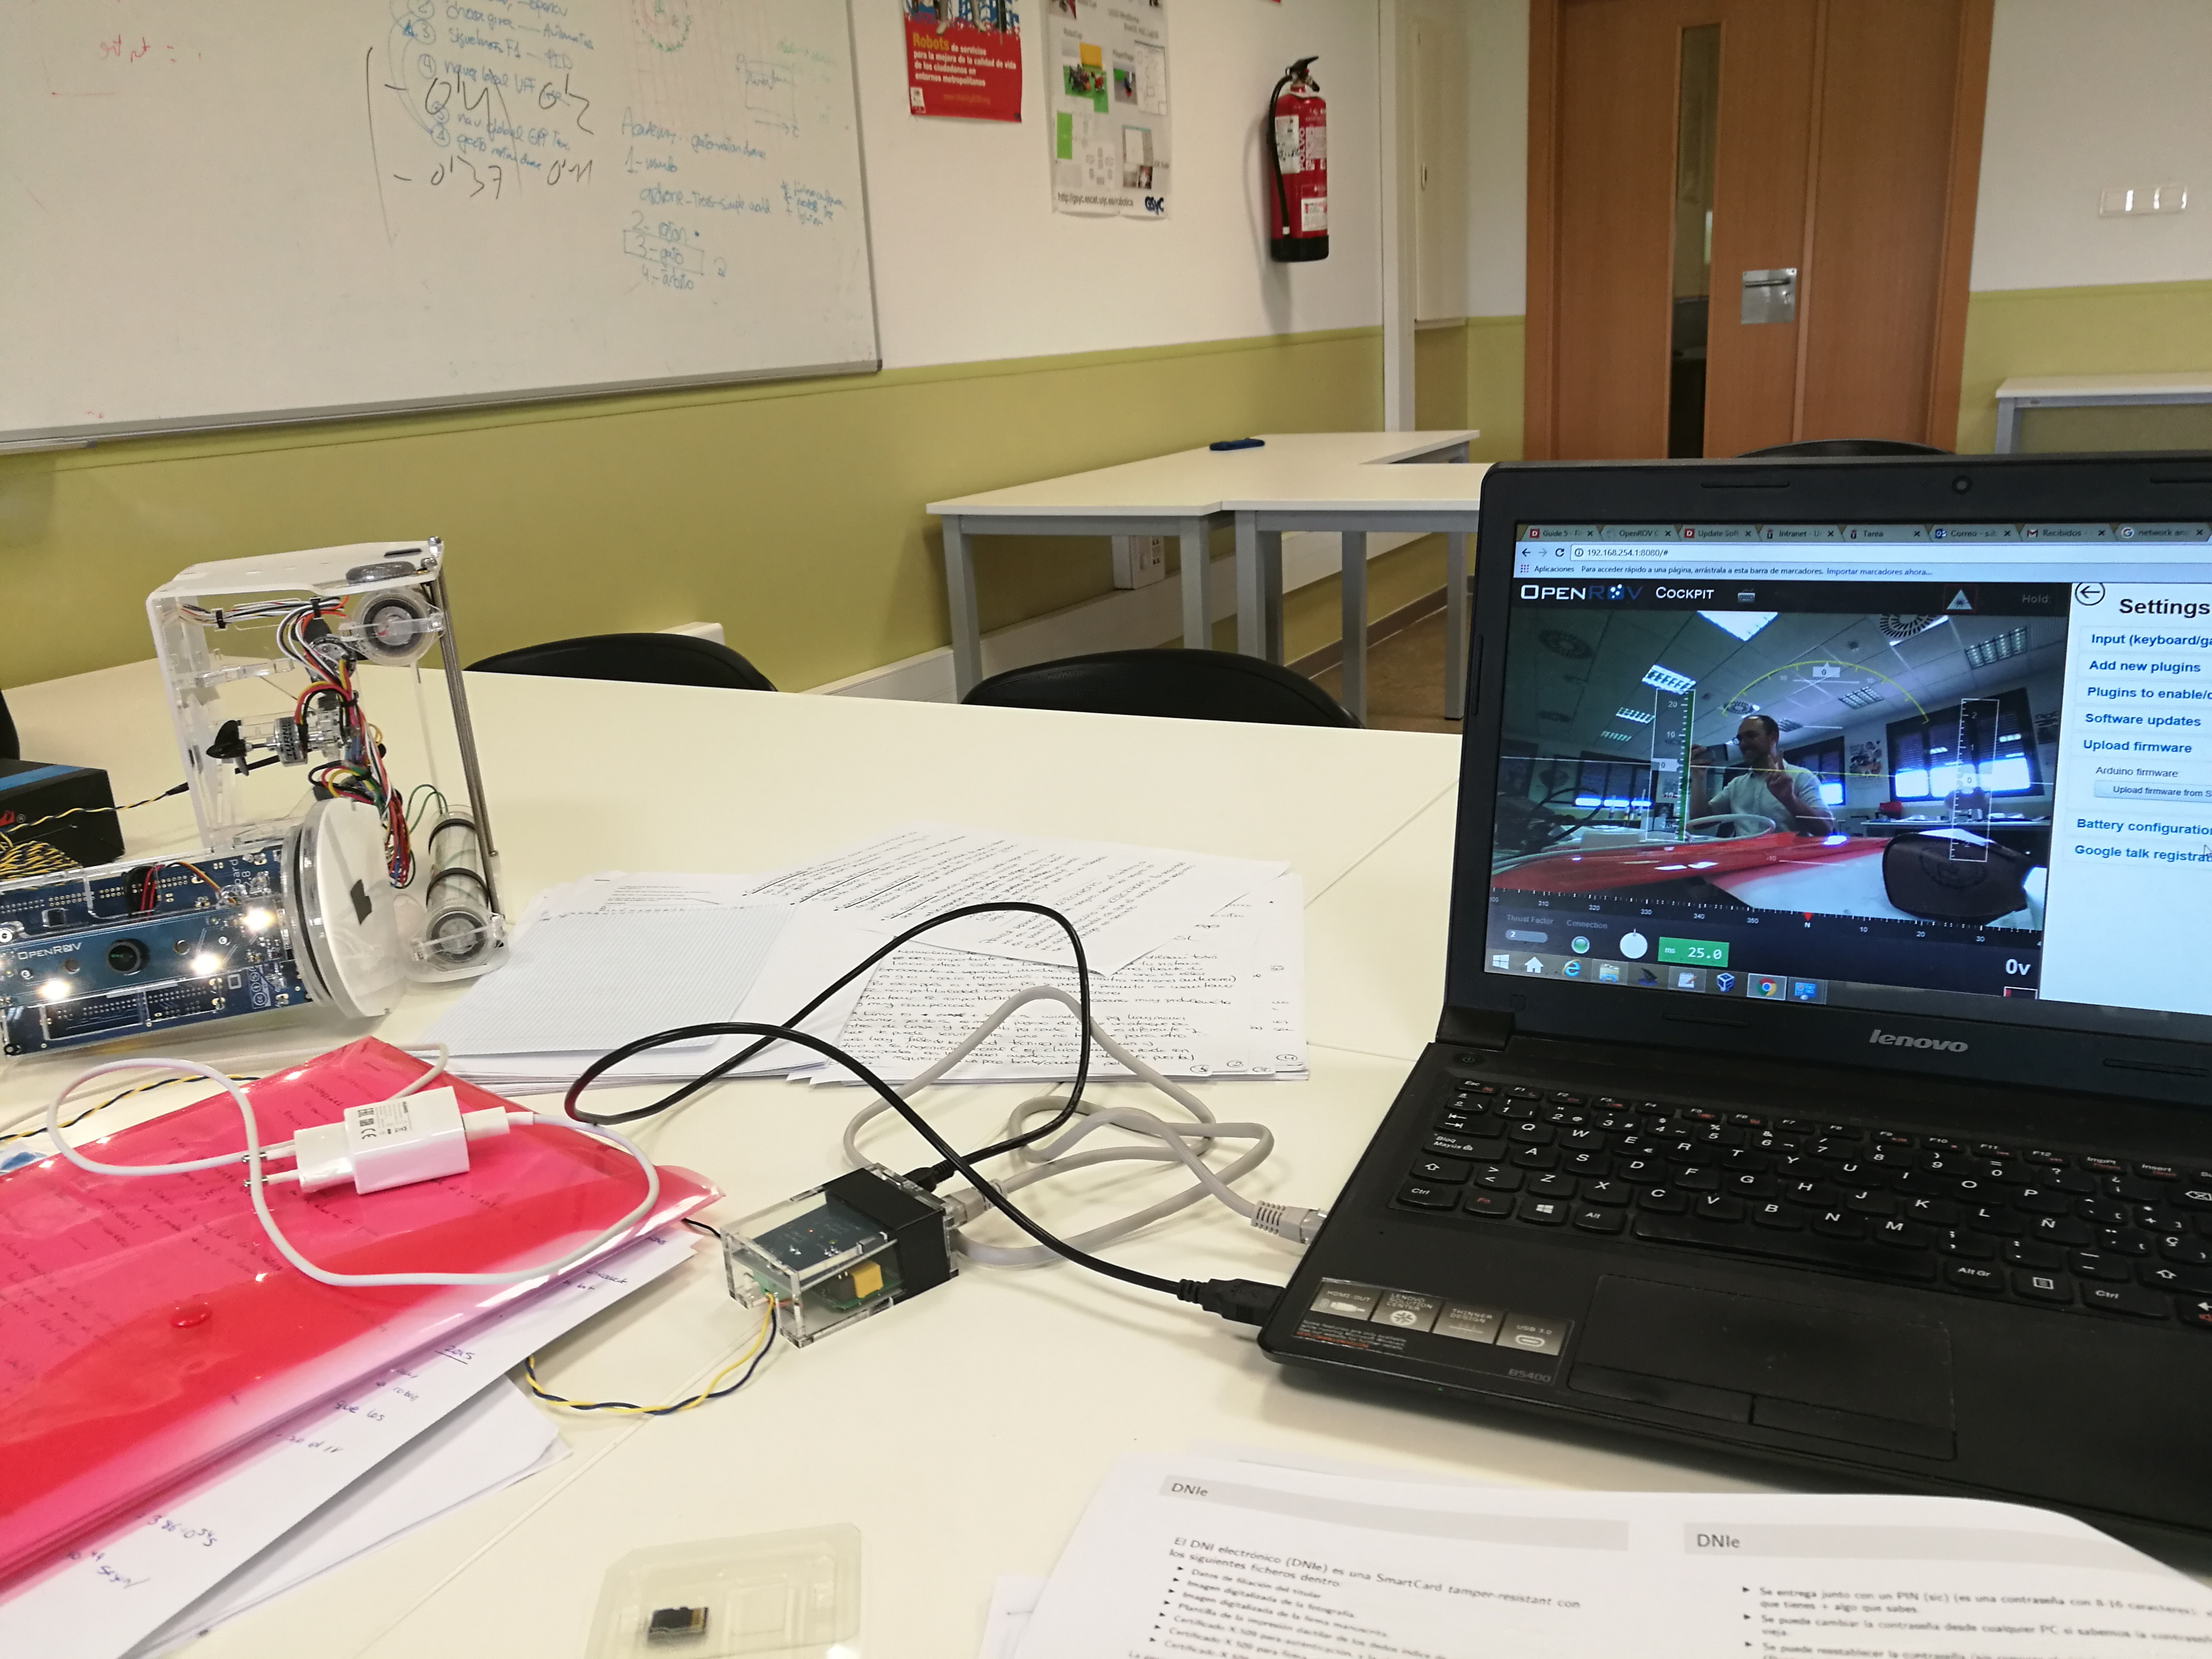
\includegraphics[width=8cm]{img/cap3/3_4/foco}
\end{center}
\caption{Foco cámara}
\label{fig:foco}
\end{figure}
    
  \subsubsection{Láser}
  \label{subsubsec:laser}
El ROV llega incorporado dos láser, los cuales tendremos que montar en el chasis de la cámara. Anteriormente estos dos láseres ya han sido soldados en la placa de la cámara, con lo que el proceso que llevaremos a cabo será su calibración y pegado.
Los puntos siempre estarán a diez centímetros de distancia uno del otro, actuando como una escala para mediciones subacuáticas.
En un papel pondremos dos “X” separados entre si diez centímetros, y colocaremos la hoja de calibración entre tres y cuatro metros de distancia de los láseres. El ROV y el folio deben colocarse a la misma altura.
Presionamos la tecla L en la web de OpenROV para encender los láseres (si volvemos a presionar esa tecla, los láseres serán desactivados).
Una vez este todo calibrado,  pegaremos con Super Glue los láseres al chasis de la cámara.
 \begin{figure}[hbtp]
  \begin{center}
    \subfigure[Distancia de los laseres]{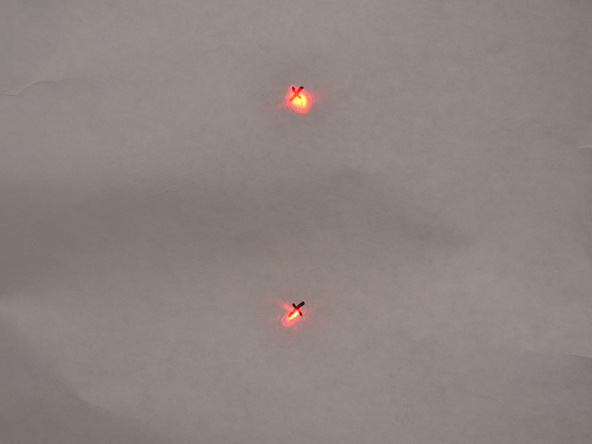
\includegraphics[width=6cm,height=5cm]{img/cap3/3_4/laseres}}
    \subfigure[Fijado del los laseres]{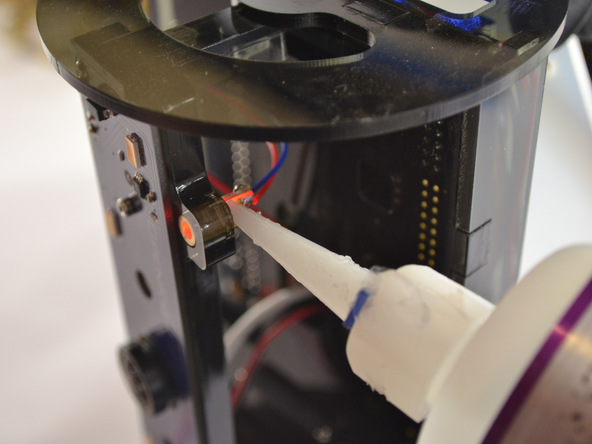
\includegraphics[width=6cm,height=5cm]{img/cap3/3_4/laser_camara}}
  \end{center}
  \caption{Láser}
  \label{fig:laser}
\end{figure}
  
\subsubsection{Motores}
\label{subsubsec:motores}
En este punto, se comprobará si las hélices giran en la dirección correcta. En la web, presionaremos la tecla de “flecha arriba” mientras miramos en que dirección giran los motores.
El motor izquierdo (amarillo) debe funcionar en sentido contrario a las agujas del reloj.
El motor derecho (azul) debe funcionar en sentido a las agujas del reloj.
\begin{figure} [hbtp]
\begin{center}
  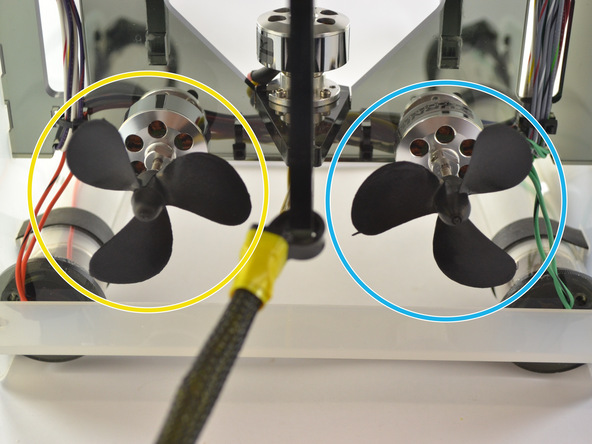
\includegraphics[width=8cm]{img/cap3/3_4/motores}
\end{center}
\caption{Motores}
\label{fig:motores}
\end{figure}

Si el giro fuera incorrecto, podemos invertirlo en la parte de “diagnóstico” de la esquina superior derecha del Cockpit. Seleccionamos la opción “inversa” del motor que queramos modificar.
%\url{https://www.youtube.com/watch?v=pck8Bpla-5w} 
\subsubsection{Tubo cilíndrico trasparente de polimetilmetacrilato}
\label{subsubsec:tubo}
El tubo cilíndrico contendrá todo el sistema hardware y software del ROV.
Lijaremos los bordes interiores del tubo principal utilizando un papel de lija de grano mediano para que la junta se ajuste en el tubo.
Limpiamos todo el polvo sobrante del proceso de lijado.
\begin{figure} [hbtp]
\begin{center}
  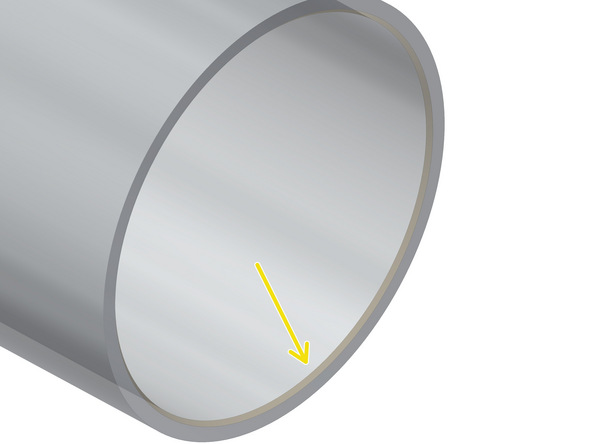
\includegraphics[width=8cm]{img/cap3/3_4/tubo}
\end{center}
\caption{Tubo}
\label{fig:tubo}
\end{figure}

\subsubsection{Tapa superior}
\label{subsubsec:tapa}
Las juntas son muy importantes para garantizar que los componentes electrónicos permanezcan secos.
Después de instalar el tubo, nos aseguramos  de que la junta se enganche a lo largo de todo el perímetro interior del tubo.
El tubo electrónico necesita el orificio de ventilación proporcionado por el émbolo para igualar la presión cuando se colocan las tapas.
\begin{figure} [hbtp]
\begin{center}
  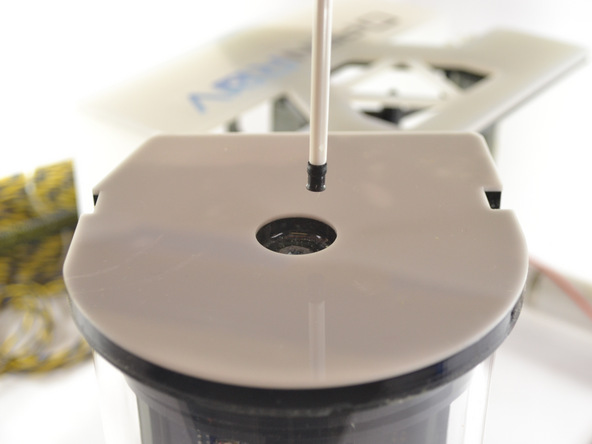
\includegraphics[width=8cm]{img/cap3/3_4/tapa_superior}
\end{center}
\caption{Tapa superior}
\label{fig:tapa_sup}
\end{figure}  
       
\subsection{Web/Cockpit}
\label{subsec:cockpit}
El ROV se maneja con Cockpit que es la interfaz de usuario y los sistemas de control para cualquier vehículo o dispositivo operado a distancia.
\\Funciona con Linux incorporado y microcontroladores para proporcionar el control tele-robot.

\begin{figure} [hbtp]
\begin{center}
  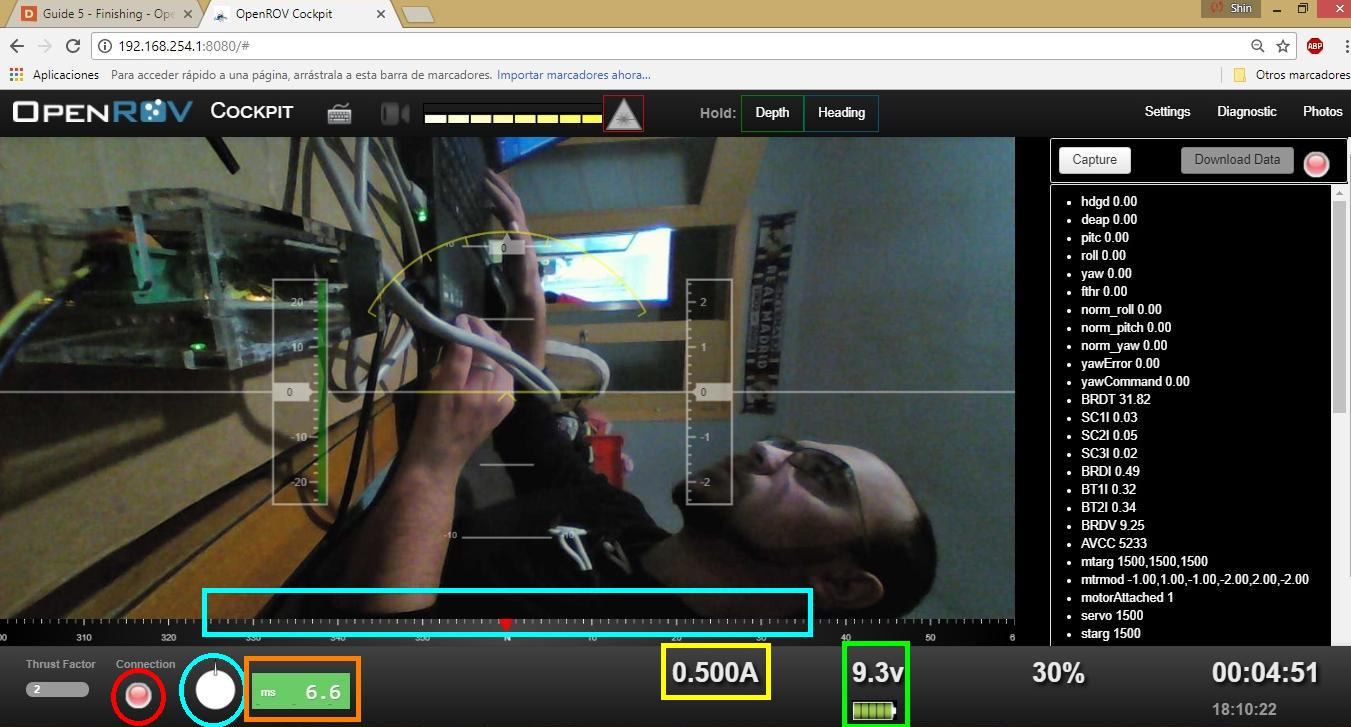
\includegraphics[width=15cm]{img/cap3/3_5/cockpit1}
\end{center}
\caption{Cockpit (1)}
\label{fig:cockpit1}
\end{figure}

\begin{itemize}
\item[\textcolor{red}{\textbullet}]Conectividad (verde = conectado)
\item[\textcolor{orange}{\textbullet}]Latencia (si hubiera algún problema mostraría +999)
\item[\textcolor{yellow}{\textbullet}]Consumo de corriente (solo los componentes electrónicos, sin incluir motores)
\item[\textcolor{green}{\textbullet}]Voltaje de la batería (para las baterías LiFe-PO4 nominales es alrededor de 9.2V, el ícono puede mostrarse medio lleno, lo cual es normal)
\item[\textcolor{blue}{\textbullet}]Brújula/rumbo (solo con IMU (Unidad de medición inercial))
\end{itemize}

\newpage
\begin{figure} [hbtp]
\begin{center}
  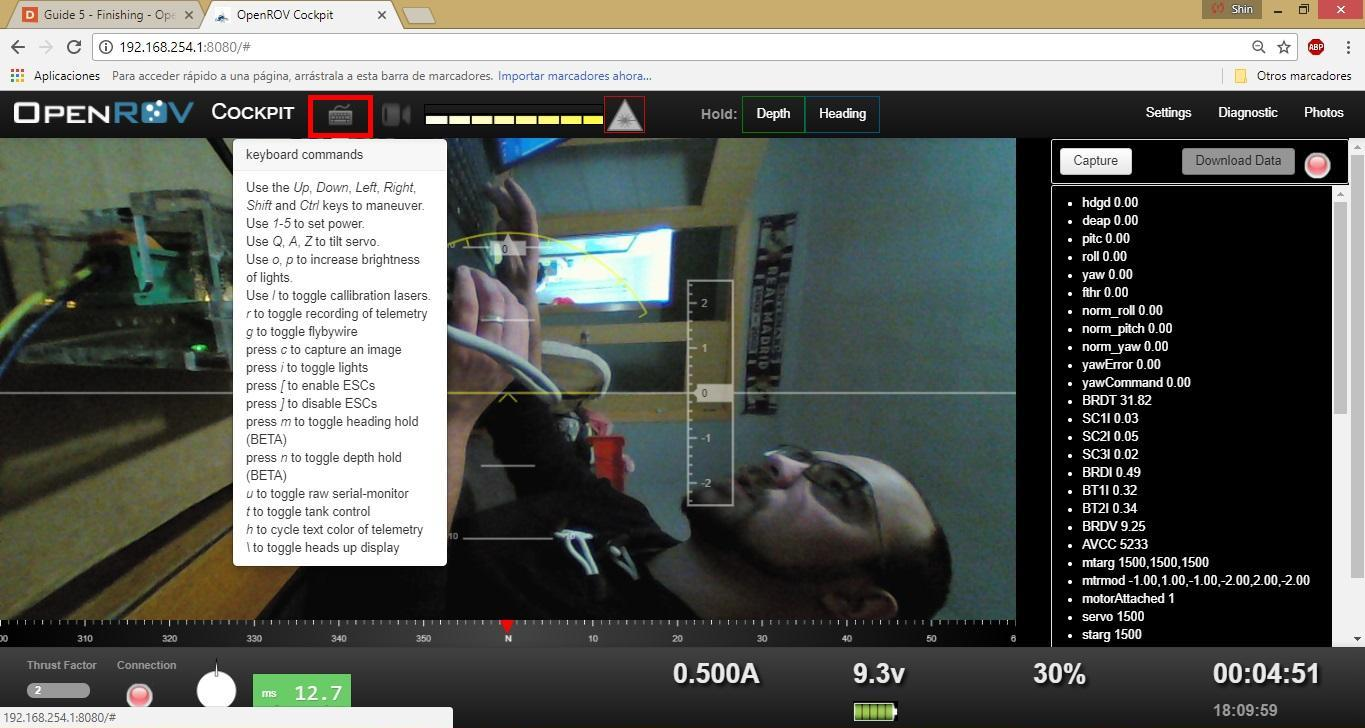
\includegraphics[width=12cm]{img/cap3/3_5/cockpit2}
\end{center}
\caption{Cockpit (2)}
\label{fig:cockpit2}
\end{figure}

\begin{itemize}
\item[\textcolor{red}{\textbullet}]Pulsamos el botón señalado en rojo (el icono del teclado) para obtener los comandos de uso del robot.
\end{itemize}


\begin{figure} [hbtp]
\begin{center}
  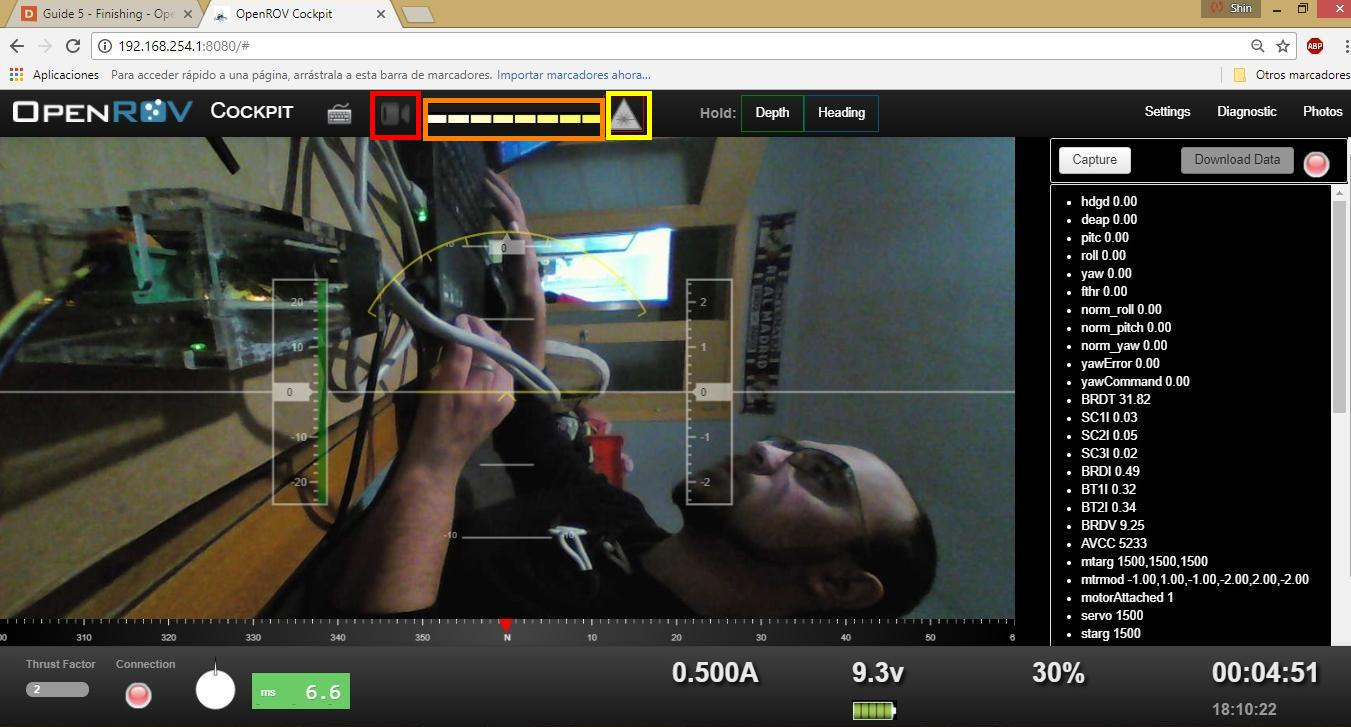
\includegraphics[width=12cm]{img/cap3/3_5/cockpit3}
\end{center}
\caption{Cockpit (3)}
\label{fig:cockpit3}
\end{figure}

\begin{itemize}
\item[\textcolor{red}{\textbullet}]Indicador de la cámara
\item[\textcolor{orange}{\textbullet}]Indicador de nivel de luz LED
\item[\textcolor{yellow}{\textbullet}]Indicador de encendido/apagado del láser
\end{itemize}

\newpage
\begin{figure} [hbtp]
\begin{center}
  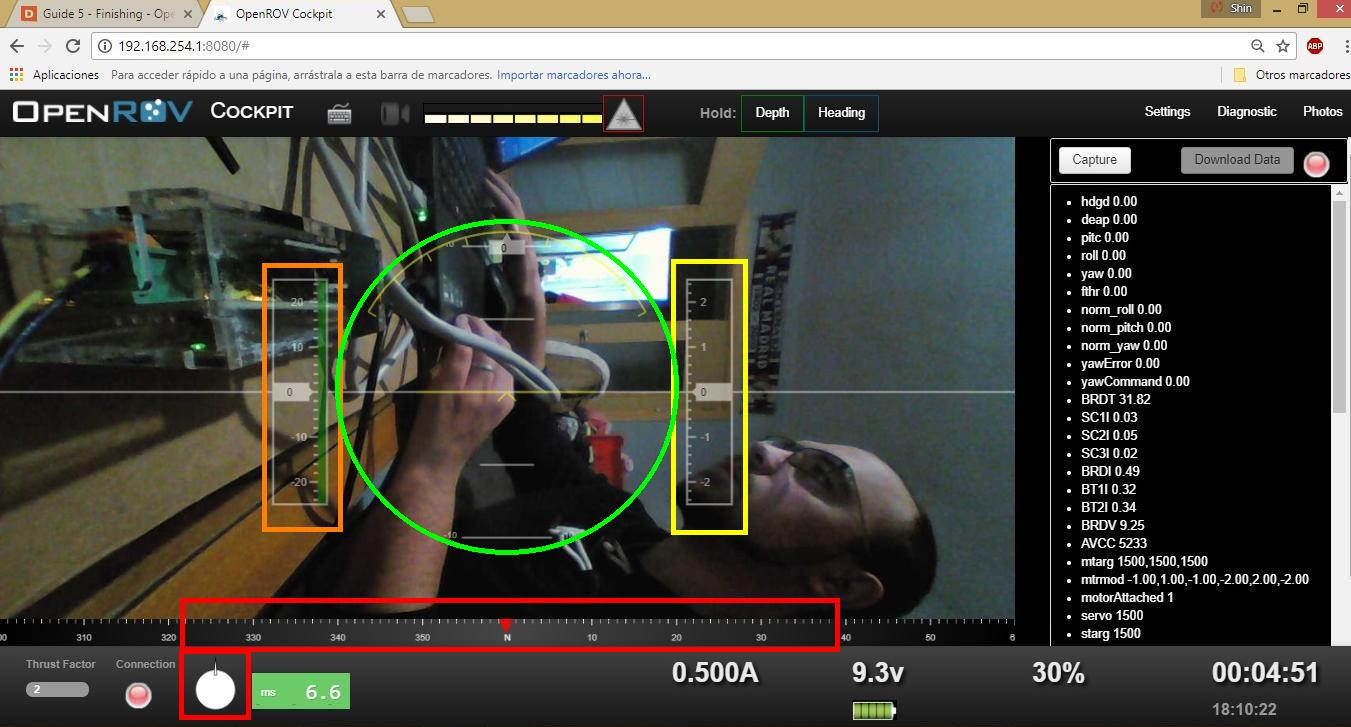
\includegraphics[width=12cm]{img/cap3/3_5/cockpit4}
\end{center}
\caption{Cockpit (4)}
\label{fig:cockpit4}
\end{figure}
\begin{itemize}
\item[\textcolor{red}{\textbullet}]Rumbo (brújula). Esto se basa en la dirección que obtiene OpenROV al inicio. Se puede calibrar alineando el ROV al norte al inicio.
\item[\textcolor{orange}{\textbullet}]Valor de empuje del motor (IMU no es necesario)
\item[\textcolor{yellow}{\textbullet}]Profundidad
\item[\textcolor{green}{\textbullet}]Horizonte artificial
\end{itemize}

\begin{figure} [hbtp]
\begin{center}
  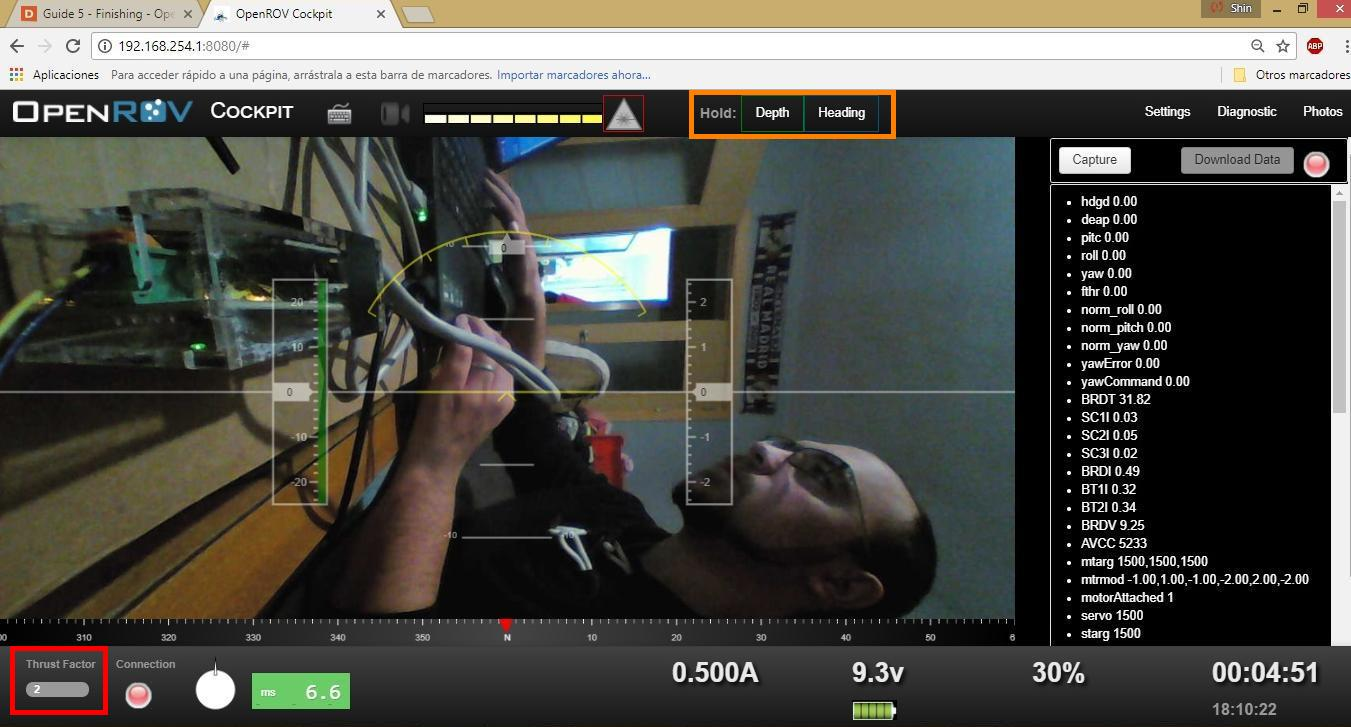
\includegraphics[width=12cm]{img/cap3/3_5/cockpit5}
\end{center}
\caption{Cockpit (5)}
\label{fig:cockpit5}
\end{figure}
\begin{itemize}
\item[\textcolor{red}{\textbullet}]La configuración de empuje (1, la más baja y 5, la más alta) cambia la potencia otorgada a los motores. El uso típico es 2-3. El uso intensivo de nivel 5 agotará las baterías rápidamente y solo se recomienda para retiros rápidos y uso intermitente.
\item[\textcolor{orange}{\textbullet}]En la parte de arriba se pueden ver los indicadores de profundidad y rumbo. Estos se alternan entre activar/desactivar para mantener la profundidad actual y/o el rumbo actual. Esta función solo funciona con la actualización profundidad/rumbo/IMU.
\end{itemize}

\begin{figure} [hbtp]
\begin{center}
  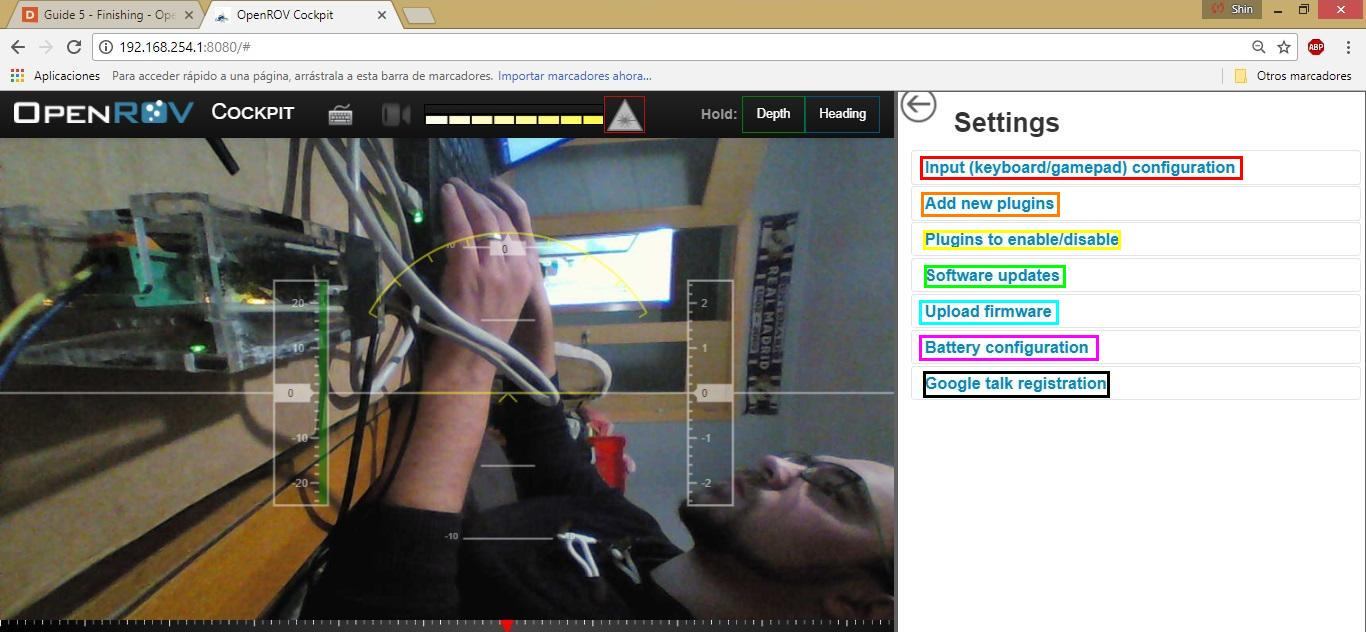
\includegraphics[width=12cm]{img/cap3/3_5/setting}
\end{center}
\caption{Ajustes}
\label{fig:settting}
\end{figure}

Panel de configuración:
\begin{itemize}
 \item Configuración de entrada: aquí puede cambiar y personalizar las combinaciones de teclas y botones.
 \item Agregar complementos nuevos: esto es para usuarios que desean usar complementos de 3ra parte (avanzados).
 \item Complementos para habilitar/deshabilitar: activa y desactiva los complementos cargados en el punto anterior (avanzado).
 \item Actualización de software: se recomendamos que siempre actualice su software. Esto también le muestra la versión de software actual.
 \item Configuración de la batería: en este punto es donde establece los voltajes mínimo y máximo de la batería.
 \item Registro de Google Talk: esta pestaña permite acceder a las funciones de redes sociales del cockpit (avanzado).
\end{itemize}

\begin{figure} [hbtp]
\begin{center}
  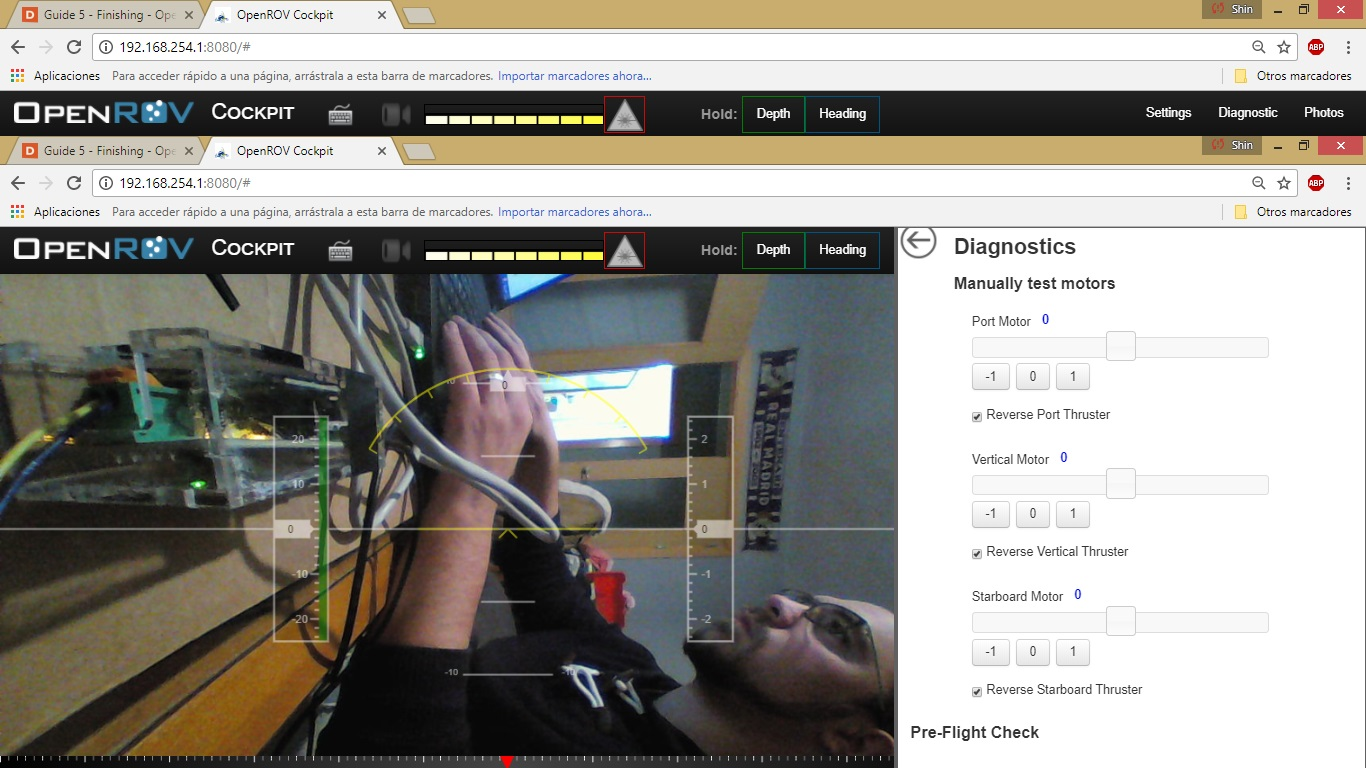
\includegraphics[width=12cm]{img/cap3/3_5/diagnostico}
\end{center}
\caption{Diagnóstico}
\label{fig:diagnostico}
\end{figure}

Panel de diagnósticos:
\begin{itemize}
 \item Probar manualmente los motores, esto se usa para hacer funcionar los motores manualmente. Este panel también sirve para invertir la dirección de un cierto motor.
 \item Pre-Flight Check es un marcador de posición por el momento.
 \item La calibración para la brújula y la profundidad cero también se encuentran en este panel.
\end{itemize}

\begin{figure} [hbtp]
\begin{center}
  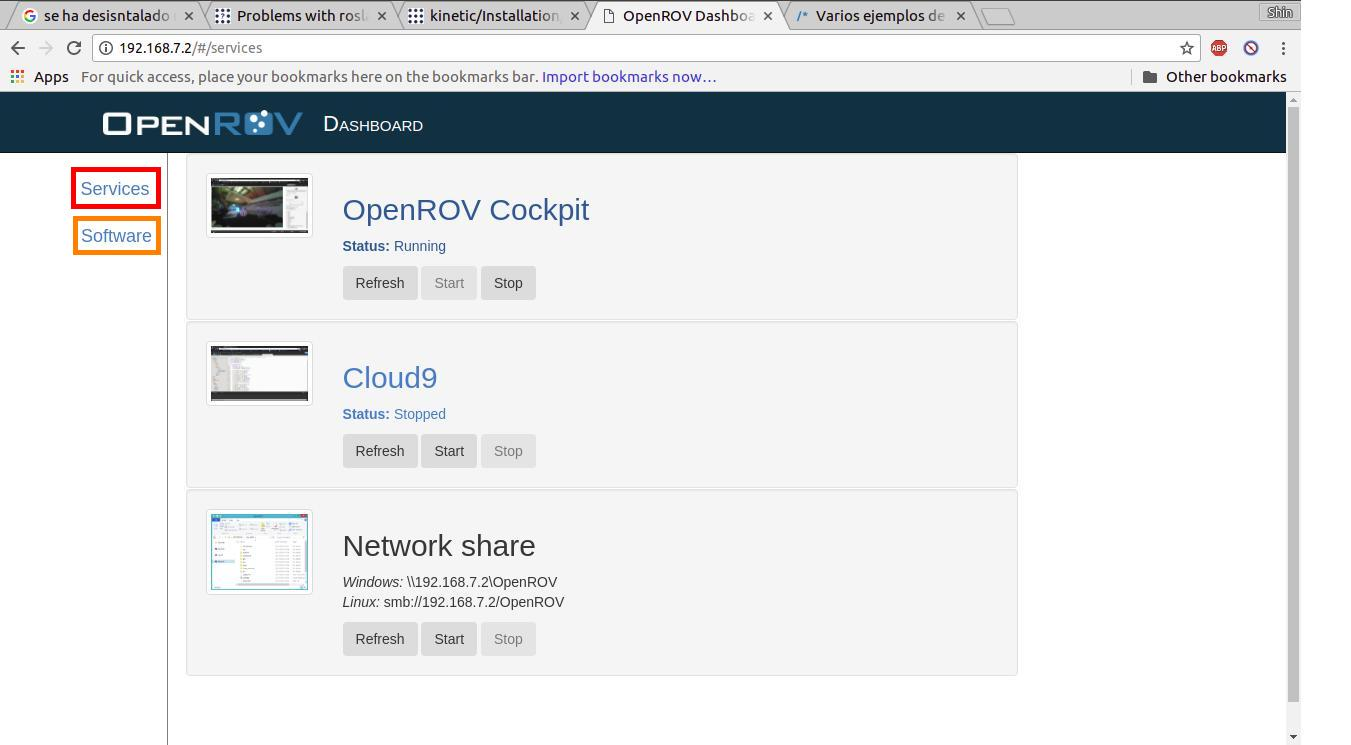
\includegraphics[width=12cm]{img/cap3/3_5/services}
\end{center}
\caption{Servicios}
\label{fig:services}
\end{figure}

El panel de configuración de OpenROV se encuentra en: 192.168.254.1

Hay dos partes:
\begin{itemize}
\item[\textcolor{red}{\textbullet}]\textbf{Servicios}: puede reiniciar la cabina, ejecutar Cloud9 para editar el código e iniciar el recurso compartido de red para acceder a los archivos en el ROV.
\item[\textcolor{orange}{\textbullet}]\textbf{Software}: puede determinar la versión de su software así como la actualización automática cuando esté conectado a Internet (software 30.0.3 y superior).
\end{itemize}

\subsection{Mantenimiento}
\label{subsec:mantenimiento}

\subsubsection{Enjuagar}
\label{subsubsec:enjuagar}
Una vez que hayamos utilizado el robot, debemos rociarlo en agua dulce después de cada inmersión, ya que es una excelente manera de mantenerlo limpio y libre de desechos y minerales.
\\Cuanto más limpia sea el agua, mejor. En orden ascendente sería:
\begin{itemize}
\item El agua desionizada como mejor opción.
\item El agua destilada.
\item El agua dulce del grifo en tercer lugar.
\end{itemize} 
  
\subsubsection{Mantenimiento de los motores}
\label{subsubsec:mantenimiento}
La parte más importante del mantenimiento posterior a la inmersión es limpiar los motores. Los imanes expuestos tienden a corroerse fácilmente. Los rodamientos también deben lubricarse y protegerse del óxido.
\begin{itemize}
\item Primero, enjuagamos los motores con agua fría.
\item Secaremos bien los motores con aire comprimido (si está disponible).
\item Inmediatamente después, volveremos a aplicar la lubricación con spray de silicona. Moveremos los motores con las manos durante algunas rotaciones para asegurarse de que los quede todo bien lubricados. Esto debe hacerse antes y después de cada inmersión.
\end{itemize}
  
\subsubsection{Secado}
\label{subsubsec:secado}
Debemos permitir que el OpenROV se seque completamente antes de guardarlo.
Usar aire comprimido o enlatado puede ayudar.
\\La apertura de los tubos de la batería y el tubo principal permitirá que el aire circule y secará la humedad que pueda haberse acumulado durante la inmersión.
  
\subsubsection{Carga de baterías}
\label{subsubsec:bateria}
Mantener las baterías en grupos de seis permitirá evitar problemas. Cargaremos los seis a la vez, y se usará todo el grupo por cada inmersión.
\\Si alguna de las tres baterías en un tubo tiene un rendimiento bajo, se puede dañar las células. Para evitar esto, podemos comprobar las baterías con un polímetro después de que se hayan cargado para asegurarse de que se carguen completamente.
\\Esto también permitirá saber cuándo es el momento de reemplazarlos, ya que eventualmente perderán su capacidad de cargar y descargar.
\\Mantener las baterías secas siempre que sea posible y sin corrosión.


\subsection{Problemas}
\label{subsec:problemas}
\subsubsection{Vaho}
\label{subsubsec:vaho}
Que el tubo principal se empañe es un problema común.

Algunas veces esta es la indicación de una fuga. Si se nota que el vaho aparece repentinamente o durante una inmersión, lo mejor será salir a la superficie y verificar si hay fugas.

El vaho se puede solucionar colocando una nueva bolsa de desecante en el tubo principal unas 1-2 horas antes de la inmersión.

Los productos químicos anti-vaho también pueden ayudar. Estos están disponibles en cualquier tienda de buceo.

\subsubsection{Video}
\label{subsubsec:video}
Muchos problemas de video pueden ocurrir durante su inmersión.

El más común es un corte o "apagón" del video. Esto se puede solucionar actualizando periódicamente la imagen del software en el BeagleBone.

\subsubsection{Control u otros problemas misceláneos}
\label{subsubsec:miscelaneos}
Mientras está en el campo, es posible que necesite restablecer el OpenROV para remediar los errores extraños y aleatorios. Para este procedimiento se debe desenchufar el cable USB de la caja del PLC y volver a enchufarlo. Este método también funciona para otros problemas de control.

\subsubsection{Pérdida aleatoria de energía de la batería}
\label{subsubsec:perdida_bateria}
A menudo, cuando hay problemas de energía, primeramente habrá que asegúrese de que todas las baterías estén en contacto entre sí y, si corresponde, el adaptador de la batería y los terminales positivo y negativo en el tubo de la batería.

Verificar el voltaje a través de los pines correspondientes del conector DB-25. Para las baterías recomendadas, esto debería ser alrededor de 9V. Se comprobara la batería positivo y negativo de los cables: Naranja / Negro-Naranja y Verde claro / Negro-Verde claro. Un pequeño trozo de alambre puede ayudar a establecer una buena conexión con el polímetro.

Además, puede verificar cada batería individual para asegurarse de que tenga el voltaje correcto.

Hay que asegurarse de mover los cables alrededor o sacudir los tubos de la batería para identificar cualquier discontinuidad.

Se puede quitar la envoltura de plástico en la parte inferior de las baterías para ayudar en un buen contacto.

\begin{figure} [hbtp]
\begin{center}
  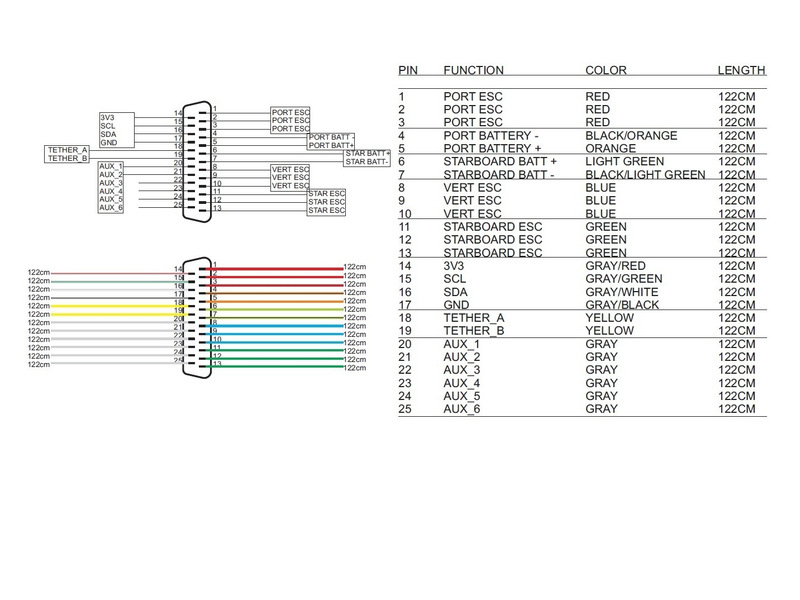
\includegraphics[width=12cm]{img/cap3/3_5/DB-25}
\end{center}
\caption{DB-25}
\label{fig:db25}
\end{figure}

\subsubsection{Enredos}
\label{subsubsec:enredos}
Los enredos es un problema muy comun que se encuentran en el este campo.

El mejor remedio es evitar la situación en absoluto. Esto se puede hacer evitando bucear en vegetación pesada.

A veces puede ser necesario tirar el OpenROV a la superficie con la correa. La correa es fuerte y puede manejar una gran cantidad de fuerza.

Hay que tener en cuenta que si se tira del OpenROV puede enredar el ROV, que es mucho más grande y difícil de desenredar. Si este es el caso, conduciremos el robot hasta nosotros o al menos hacia la superficie donde se puede recuperar. Luego, desconectaremos el cable USB del PLC y se tirará del ROV.

Siempre podemos cortar y volver a soldar la correa utilizando un tubo termorretráctil si fuese necesario.

\subsubsection{Inundación del tubo principal}
\label{subsubsec:inundacion_tubo}
Este puede ser el mayor problema al que nos podemos enfrentar, por ello, lo primero que habría que realizar sería desconectar la alimentación del ROV (esto evitará que la electrólisis corroa los componentes electrónicos). Para hacer esto, desenchufamos el cable USB y retiraremos las baterías.

Si el agua que inundó el tubo no era agua dulce, enjuagamos los componentes electrónicos que se mojaron en agua dulce (desionizada> destilada> agua del grifo) para diluir y eliminar los minerales del área que se inundó.

Quitaremos los componentes electrónicos para exponer tantas superficies como sea posible.

Se enjuagará las áreas afectadas una vez más.

Secaremos bien cada una de las piezas de la electrónica. El aire comprimido puede ayudar.

Se colocaran todos los componentes electrónicos afectados en un lugar seco. Es útil tener una bolsa de llena de arroz o desecante.

Cuando vuelva a armar todo, inspeccionamos para detectar corrosión. Si vemos alguno, a menudo se puede quitar con un cepillo de dientes. La corrosión no significa necesariamente un fallo, pero es bueno eliminar lo que se pueda.